\documentclass{article}
\usepackage{fullpage}
\usepackage{amsmath,amssymb}
\usepackage{amsthm}
\usepackage{graphicx}
\usepackage{natbib}
\usepackage[hidelinks]{hyperref}
\usepackage{bm}
\usepackage{todonotes}
\usepackage{authblk}
\renewcommand\Affilfont{\itshape\small}

\newcommand{\peter}[1]{\todo[color=green!40]{Peter: #1}}
\newcommand{\erick}[1]{\todo[color=purple!40]{Erick: #1}}

\newcommand{\E}{\mathbb{E}}
\renewcommand{\P}{\mathbb{P}}
\newcommand{\calS}{\mathcal{S}}  % set of states
\newcommand{\calT}{\mathcal{T}}  % set of transition triples
\newcommand{\calP}{\mathcal{P}}  % set of selection pairs
\newcommand{\calM}{\mathcal{M}}  % set of potential mutations
\newcommand{\nA}{\mbox{A}}  % nucleotides:
\newcommand{\nC}{\mbox{C}}
\newcommand{\nG}{\mbox{G}}
\newcommand{\nT}{\mbox{T}}
\newcommand{\nS}{\mbox{S}} % C or G
\newcommand{\nW}{\mbox{W}} % A or T
\newcommand{\nR}{\mbox{R}} % purine, A or G
\newcommand{\nY}{\mbox{Y}} % pyrimidine, C or T
\newcommand{\join}{\oplus}  % concatenation
\newcommand{\st}{\colon}  % such that
\newcommand{\var}{\mathop{\mbox{var}}}
\newcommand{\cov}{\mathop{\mbox{cov}}}
\newcommand{\given}{\;\mid\;}
\newcommand{\like}{\mathcal L}
\newcommand{\loglike}{\ell}
\newcommand{\alike}{\widetilde{\like}}
\newcommand{\aloglike}{\widetilde{\loglike}}

\newcommand{\APOBEC}{\text{\tiny APOBEC}}
\newcommand{\AID}{\text{\tiny AID}}

\theoremstyle{plain}
\newtheorem{theorem}{Theorem}
\newtheorem{lemma}{Lemma}
\theoremstyle{definition}
\newtheorem{example}{Example}[section]

\bibliographystyle{plainnat}

% http://bytesizebio.net/2013/03/11/adding-supplementary-tables-and-figures-in-latex/
\newcommand{\beginsupplement}{%
        \setcounter{table}{0}
        \renewcommand{\thetable}{S\arabic{table}}%
        \setcounter{figure}{0}
        \renewcommand{\thefigure}{S\arabic{figure}}%
     }

% Responses to reviews
\usepackage{lineno, hyperref}
% \usepackage[hypertexnames=false]{hyperref}   % not working correctly
% \usepackage{latexml}

\linenumbers


%%%%%  PUT THIS IN HEADER OF FILE
% % Responses to reviews:
% \usepackage{lineno, hyperref}
% \usepackage[hypertexnames=false]{hyperref}   % not working correctly
% \usepackage{latexml}

\linenumbers


%%%%%  PUT THIS IN HEADER OF FILE
% % Responses to reviews:
% \usepackage{lineno, hyperref}
% \usepackage[hypertexnames=false]{hyperref}   % not working correctly
% \usepackage{latexml}

\linenumbers


%%%%%  PUT THIS IN HEADER OF FILE
% % Responses to reviews:
% \input{review-response-commands}
% % set this to show line numbers and include responses to reviews or not
% \newif\ifreviewresponses
% \reviewresponsestrue  % include them
% % \reviewresponsesfalse  % don't include them
% \newcommand{\responsefile}{pbio-reviews-19sept12-responses.tex}  % name of the review reponses file

% counters for reviewer points
%% instead do reviewer labels
% \newcounter{reviewer}
% \setcounter{reviewer}{0}
\newcommand{\thereviewer}{}
\newcounter{point}
\setcounter{point}{0}

% pass in to \reviewersection the label for this reviewer (i.e. \reviewersection{1} or \reviewersection{AE})
\newcommand{\reviewersection}[1]{\renewcommand{\thereviewer}{#1}
                  \setcounter{point}{0}
                  \section*{Reviewer \thereviewer:}}
% drawing from from http://tex.stackexchange.com/questions/2317/latex-style-or-macro-for-detailed-response-to-referee-report
%% arguments to \point are (name of the point, optional) and (content)
\newenvironment{point}[1]
        { \refstepcounter{point} \bigskip \hrule \medskip \noindent 
                \slshape {\fontseries{b}\selectfont (\thereviewer.\thepoint) #1} }
        { }
\newcommand{\reply}{\normalfont \medskip \noindent \textbf{Reply}:\ }   

% use this command in the text where a change addressing a reviewer point has occurred
% e.g. \revpoint{1}{3} for reviewer 1, point 3
\newcommand{\revpoint}[2]{\hypertarget{llineno:rev#1:#2}{\linelabel{rr:rev#1:#2}}}
% and this one to refer to such a location, e.g. \revreffull{1}{3}
\newcommand{\revreffull}[2]{{(p.\ \hyperlink{llineno:rev#1:#2}{\pageref{rr:rev#1:#2}, l.\ \lineref{rr:rev#1:#2}})}}
% but this version fills in reviewer and point automatically if called in the appropriate part of the reviews
\newcommand{\revref}{\revreffull{\thereviewer}{\thepoint}}
% NOTE: should call \revref{} with empty brackets after to get a space afterwards if desired: http://tex.stackexchange.com/questions/31091/space-after-latex-commands

% or, this one to refer to a named linelabel
% e.g. if in the text there is a \llabel{approx_eqn_point}
% refer to it with \llname{approx_eqn_point}
\newcommand{\llabel}[1]{\hypertarget{ll:#1}{\linelabel{#1}}}
\newcommand{\llname}[1]{{(p.\ \hyperlink{ll:#1}{\pageref{#1}, l.\ \lineref{#1}})}}

% put \includereviews() where the reviews are to appear (at the end?)
\newcommand{\includereviews}{
    \ifreviewresponses
    \clearpage
    \setcounter{page}{1}
    \setcounter{section}{0}
    \setcounter{subsection}{0}
    \nolinenumbers
    % \begin{center}
    %   {\LARGE \bf Response to Reviews}
    % \end{center}
    \input{\responsefile}
    \fi
}

% Useful shortcuts ;) that demonstrate how to use the macros.
\newcommand{\rollover}{ \reply{The reviewer makes an excellent point that we have missed out entirely.  We have made all the changes suggested, down to the minutiae \revref.} }
\newcommand{\playdead}{ \reply{The reviewer makes an excellent point.  We have made an utterly trivial change {\revref} that we think deals entirely with the concern raised.} }
                                                                                                         
% from http://tex.stackexchange.com/questions/43648/why-doesnt-lineno-number-a-paragraph-when-it-is-followed-by-an-align-equation/55297#55297
\ifcsname{patchAmsMathEnvironmentForLineno}\endcsname
    \newcommand*\patchAmsMathEnvironmentForLineno[1]{%                                                       
      \expandafter\let\csname old#1\expandafter\endcsname\csname #1\endcsname                                
      \expandafter\let\csname oldend#1\expandafter\endcsname\csname end#1\endcsname                          
      \renewenvironment{#1}%                                                                                 
         {\linenomath\csname old#1\endcsname}%                                                               
         {\csname oldend#1\endcsname\endlinenomath}}%                                                        
    \newcommand*\patchBothAmsMathEnvironmentsForLineno[1]{%                                                  
      \patchAmsMathEnvironmentForLineno{#1}%                                                                 
      \patchAmsMathEnvironmentForLineno{#1*}}%                                                               
    \AtBeginDocument{%                                                                                       
    \patchBothAmsMathEnvironmentsForLineno{equation}%                                                        
    \patchBothAmsMathEnvironmentsForLineno{align}%                                                           
    \patchBothAmsMathEnvironmentsForLineno{flalign}%                                                         
    \patchBothAmsMathEnvironmentsForLineno{alignat}%                                                         
    \patchBothAmsMathEnvironmentsForLineno{gather}%                                                          
    \patchBothAmsMathEnvironmentsForLineno{multline}%                                                        
\fi

% % set this to show line numbers and include responses to reviews or not
% \newif\ifreviewresponses
% \reviewresponsestrue  % include them
% % \reviewresponsesfalse  % don't include them
% \newcommand{\responsefile}{pbio-reviews-19sept12-responses.tex}  % name of the review reponses file

% counters for reviewer points
%% instead do reviewer labels
% \newcounter{reviewer}
% \setcounter{reviewer}{0}
\newcommand{\thereviewer}{}
\newcounter{point}
\setcounter{point}{0}

% pass in to \reviewersection the label for this reviewer (i.e. \reviewersection{1} or \reviewersection{AE})
\newcommand{\reviewersection}[1]{\renewcommand{\thereviewer}{#1}
                  \setcounter{point}{0}
                  \section*{Reviewer \thereviewer:}}
% drawing from from http://tex.stackexchange.com/questions/2317/latex-style-or-macro-for-detailed-response-to-referee-report
%% arguments to \point are (name of the point, optional) and (content)
\newenvironment{point}[1]
        { \refstepcounter{point} \bigskip \hrule \medskip \noindent 
                \slshape {\fontseries{b}\selectfont (\thereviewer.\thepoint) #1} }
        { }
\newcommand{\reply}{\normalfont \medskip \noindent \textbf{Reply}:\ }   

% use this command in the text where a change addressing a reviewer point has occurred
% e.g. \revpoint{1}{3} for reviewer 1, point 3
\newcommand{\revpoint}[2]{\hypertarget{llineno:rev#1:#2}{\linelabel{rr:rev#1:#2}}}
% and this one to refer to such a location, e.g. \revreffull{1}{3}
\newcommand{\revreffull}[2]{{(p.\ \hyperlink{llineno:rev#1:#2}{\pageref{rr:rev#1:#2}, l.\ \lineref{rr:rev#1:#2}})}}
% but this version fills in reviewer and point automatically if called in the appropriate part of the reviews
\newcommand{\revref}{\revreffull{\thereviewer}{\thepoint}}
% NOTE: should call \revref{} with empty brackets after to get a space afterwards if desired: http://tex.stackexchange.com/questions/31091/space-after-latex-commands

% or, this one to refer to a named linelabel
% e.g. if in the text there is a \llabel{approx_eqn_point}
% refer to it with \llname{approx_eqn_point}
\newcommand{\llabel}[1]{\hypertarget{ll:#1}{\linelabel{#1}}}
\newcommand{\llname}[1]{{(p.\ \hyperlink{ll:#1}{\pageref{#1}, l.\ \lineref{#1}})}}

% put \includereviews() where the reviews are to appear (at the end?)
\newcommand{\includereviews}{
    \ifreviewresponses
    \clearpage
    \setcounter{page}{1}
    \setcounter{section}{0}
    \setcounter{subsection}{0}
    \nolinenumbers
    % \begin{center}
    %   {\LARGE \bf Response to Reviews}
    % \end{center}
    \input{\responsefile}
    \fi
}

% Useful shortcuts ;) that demonstrate how to use the macros.
\newcommand{\rollover}{ \reply{The reviewer makes an excellent point that we have missed out entirely.  We have made all the changes suggested, down to the minutiae \revref.} }
\newcommand{\playdead}{ \reply{The reviewer makes an excellent point.  We have made an utterly trivial change {\revref} that we think deals entirely with the concern raised.} }
                                                                                                         
% from http://tex.stackexchange.com/questions/43648/why-doesnt-lineno-number-a-paragraph-when-it-is-followed-by-an-align-equation/55297#55297
\ifcsname{patchAmsMathEnvironmentForLineno}\endcsname
    \newcommand*\patchAmsMathEnvironmentForLineno[1]{%                                                       
      \expandafter\let\csname old#1\expandafter\endcsname\csname #1\endcsname                                
      \expandafter\let\csname oldend#1\expandafter\endcsname\csname end#1\endcsname                          
      \renewenvironment{#1}%                                                                                 
         {\linenomath\csname old#1\endcsname}%                                                               
         {\csname oldend#1\endcsname\endlinenomath}}%                                                        
    \newcommand*\patchBothAmsMathEnvironmentsForLineno[1]{%                                                  
      \patchAmsMathEnvironmentForLineno{#1}%                                                                 
      \patchAmsMathEnvironmentForLineno{#1*}}%                                                               
    \AtBeginDocument{%                                                                                       
    \patchBothAmsMathEnvironmentsForLineno{equation}%                                                        
    \patchBothAmsMathEnvironmentsForLineno{align}%                                                           
    \patchBothAmsMathEnvironmentsForLineno{flalign}%                                                         
    \patchBothAmsMathEnvironmentsForLineno{alignat}%                                                         
    \patchBothAmsMathEnvironmentsForLineno{gather}%                                                          
    \patchBothAmsMathEnvironmentsForLineno{multline}%                                                        
\fi

% % set this to show line numbers and include responses to reviews or not
% \newif\ifreviewresponses
% \reviewresponsestrue  % include them
% % \reviewresponsesfalse  % don't include them
% \newcommand{\responsefile}{pbio-reviews-19sept12-responses.tex}  % name of the review reponses file

% counters for reviewer points
%% instead do reviewer labels
% \newcounter{reviewer}
% \setcounter{reviewer}{0}
\newcommand{\thereviewer}{}
\newcounter{point}
\setcounter{point}{0}

% pass in to \reviewersection the label for this reviewer (i.e. \reviewersection{1} or \reviewersection{AE})
\newcommand{\reviewersection}[1]{\renewcommand{\thereviewer}{#1}
                  \setcounter{point}{0}
                  \section*{Reviewer \thereviewer:}}
% drawing from from http://tex.stackexchange.com/questions/2317/latex-style-or-macro-for-detailed-response-to-referee-report
%% arguments to \point are (name of the point, optional) and (content)
\newenvironment{point}[1]
        { \refstepcounter{point} \bigskip \hrule \medskip \noindent 
                \slshape {\fontseries{b}\selectfont (\thereviewer.\thepoint) #1} }
        { }
\newcommand{\reply}{\normalfont \medskip \noindent \textbf{Reply}:\ }   

% use this command in the text where a change addressing a reviewer point has occurred
% e.g. \revpoint{1}{3} for reviewer 1, point 3
\newcommand{\revpoint}[2]{\hypertarget{llineno:rev#1:#2}{\linelabel{rr:rev#1:#2}}}
% and this one to refer to such a location, e.g. \revreffull{1}{3}
\newcommand{\revreffull}[2]{{(p.\ \hyperlink{llineno:rev#1:#2}{\pageref{rr:rev#1:#2}, l.\ \lineref{rr:rev#1:#2}})}}
% but this version fills in reviewer and point automatically if called in the appropriate part of the reviews
\newcommand{\revref}{\revreffull{\thereviewer}{\thepoint}}
% NOTE: should call \revref{} with empty brackets after to get a space afterwards if desired: http://tex.stackexchange.com/questions/31091/space-after-latex-commands

% or, this one to refer to a named linelabel
% e.g. if in the text there is a \llabel{approx_eqn_point}
% refer to it with \llname{approx_eqn_point}
\newcommand{\llabel}[1]{\hypertarget{ll:#1}{\linelabel{#1}}}
\newcommand{\llname}[1]{{(p.\ \hyperlink{ll:#1}{\pageref{#1}, l.\ \lineref{#1}})}}

% put \includereviews() where the reviews are to appear (at the end?)
\newcommand{\includereviews}{
    \ifreviewresponses
    \clearpage
    \setcounter{page}{1}
    \setcounter{section}{0}
    \setcounter{subsection}{0}
    \nolinenumbers
    % \begin{center}
    %   {\LARGE \bf Response to Reviews}
    % \end{center}
    \input{\responsefile}
    \fi
}

% Useful shortcuts ;) that demonstrate how to use the macros.
\newcommand{\rollover}{ \reply{The reviewer makes an excellent point that we have missed out entirely.  We have made all the changes suggested, down to the minutiae \revref.} }
\newcommand{\playdead}{ \reply{The reviewer makes an excellent point.  We have made an utterly trivial change {\revref} that we think deals entirely with the concern raised.} }
                                                                                                         
% from http://tex.stackexchange.com/questions/43648/why-doesnt-lineno-number-a-paragraph-when-it-is-followed-by-an-align-equation/55297#55297
\ifcsname{patchAmsMathEnvironmentForLineno}\endcsname
    \newcommand*\patchAmsMathEnvironmentForLineno[1]{%                                                       
      \expandafter\let\csname old#1\expandafter\endcsname\csname #1\endcsname                                
      \expandafter\let\csname oldend#1\expandafter\endcsname\csname end#1\endcsname                          
      \renewenvironment{#1}%                                                                                 
         {\linenomath\csname old#1\endcsname}%                                                               
         {\csname oldend#1\endcsname\endlinenomath}}%                                                        
    \newcommand*\patchBothAmsMathEnvironmentsForLineno[1]{%                                                  
      \patchAmsMathEnvironmentForLineno{#1}%                                                                 
      \patchAmsMathEnvironmentForLineno{#1*}}%                                                               
    \AtBeginDocument{%                                                                                       
    \patchBothAmsMathEnvironmentsForLineno{equation}%                                                        
    \patchBothAmsMathEnvironmentsForLineno{align}%                                                           
    \patchBothAmsMathEnvironmentsForLineno{flalign}%                                                         
    \patchBothAmsMathEnvironmentsForLineno{alignat}%                                                         
    \patchBothAmsMathEnvironmentsForLineno{gather}%                                                          
    \patchBothAmsMathEnvironmentsForLineno{multline}%                                                        
\fi

% set this to show line numbers and include responses to reviews or not
\newif\ifreviewresponses
\reviewresponsestrue  % include them
% \reviewresponsesfalse  % don't include them
\newcommand{\responsefile}{reviews/reviews.v1.tex}  % name of the review responses file

\newif\ifsubmission
\submissiontrue
% \submissionfalse
\ifsubmission
    % % stuff for submission
    \usepackage{lineno}
    % allow line numbers around math environments
    % from https://tex.stackexchange.com/questions/43648/why-doesnt-lineno-number-a-paragraph-when-it-is-followed-by-an-align-equation
        \newcommand*\patchAmsMathEnvironmentForLineno[1]{%
          \expandafter\let\csname old#1\expandafter\endcsname\csname #1\endcsname
          \expandafter\let\csname oldend#1\expandafter\endcsname\csname end#1\endcsname
          \renewenvironment{#1}%
             {\linenomath\csname old#1\endcsname}%
             {\csname oldend#1\endcsname\endlinenomath}}%
        \newcommand*\patchBothAmsMathEnvironmentsForLineno[1]{%
          \patchAmsMathEnvironmentForLineno{#1}%
          \patchAmsMathEnvironmentForLineno{#1*}}%
        \AtBeginDocument{%
        \patchBothAmsMathEnvironmentsForLineno{equation}%
        \patchBothAmsMathEnvironmentsForLineno{align}%
        \patchBothAmsMathEnvironmentsForLineno{flalign}%
        \patchBothAmsMathEnvironmentsForLineno{alignat}%
        \patchBothAmsMathEnvironmentsForLineno{gather}%
        \patchBothAmsMathEnvironmentsForLineno{multline}%
        }
\else
    % for the nice version
\fi



\begin{document}


% TODO after submission: think about the BCR parameter regime.


\title{Enabling inference for context-dependent models of mutation by bounding the propagation of dependency}
\author[2,3,4,5]{Frederick A Matsen IV}
\author[1,*]{Peter L Ralph}

\affil[1]{Institute of Ecology \& Evolution, Department of Biology, University of Oregon}
\affil[2]{Computational Biology Program, Fred Hutchinson Cancer Research Center, United States}
\affil[3]{Department of Genome Sciences, University of Washington}
\affil[4]{Department of Statistics, University of Washington}
\affil[5]{Howard Hughes Medical Institute}
\affil[*]{Corresponding author: plr@uoregon.edu}


\maketitle

\begin{abstract}
    Although the rates at which positions in the genome mutate
    are known to depend not only on the nucleotide to be mutated,
    but also on neighboring nucleotides,
    it remains challenging to do phylogenetic inference
    using models of context-dependent mutation.
    In these models,
    the effects of one mutation may in principle propagate
    to faraway locations,
    making it difficult to compute exact likelihoods.
    This paper shows how to use bounds on the propagation of dependency
    to compute likelihoods of mutation of a given segment of genome
    by marginalizing over sufficiently long flanking sequence.
    This can be used for maximum likelihood or Bayesian inference.
    Protocols examining residuals and iterative model refinement
    are also discussed.
    Tools for efficiently working with these models
    are provided in an R package,
    that could be used in other applications.
    The method is used to examine context dependence of mutations
    since the common ancestor of humans and chimpanzee.
\end{abstract}

\section*{Introduction}

Early models of DNA sequence mutation
assumed that each nucleotide was equally likely to mutate
into any other nucleotide \citep{jukes1969evolution}.
These were followed by others that incorporated differences
in the mutation process, such as higher transition to transversion ratio
\citep{hasegawa1985dating,felsenstein1996hidden}.
Although the rates of mutation of a nucleotide
are known to depend on not only the nucleotide itself
but also nearby sequence context \citep{seplyarskiy2021population},
it is difficult to take this context into account when performing inference.

This situation from biological sequence analysis
is an example of a more commonly encountered class of models in statistics:
a lattice of sites,
with each site taking one of a finite collection of possible states,
and whose stochastic, temporal evolution is Markov and governed by a set of local rules.
For instance, at each site may sit
a nucleotide whose mutation rate depends on physical properties determined by the nearby DNA sequence;
a cell whose infection status depends on the state of its neighbors;
or a particle whose spin is perturbed by external noise to a state whose distribution depends on the local energy configuration.
Practical use of such models often requires
inferring transition rules
based on observations of the system at several time points,
or of several states evolved along a tree from a single starting point.
This paper concerns scalable methods for doing inference under such models using observations.

The situation is similar to the widely-studied problem of inference based on observation
of a single instance of a Markov random field,
and in many cases reduces to this if we only observe the system at one time point at stationarity.
These are used, for instance, in spatial statistics \citep{besag1972nearestneighbour,gelfand2010handbook}
and image reconstruction \citep{geman1984stochastic,besag1986statistical}.
The conditioning method we consider here
is similar to the ``coding'' scheme introduced by \citet{besag1974spatial},
that conditions on a set of sites that makes the remaining observations independent;
% (thanks to the Gibbs property);
consistency of such methods has been shown by \citet{comets1992consistency} and reviewed by \citet{larribe2011composite}.
A good review of recent statistical techniques is given by \citet{friel2012bayesian}.


In the context of genomics,
it is well-known that certain short nucleotide sequences
are in many organisms much more, or less, abundant than expected by chance \citep{burge1992underrepresentation},
due to the combined effects of context dependence of the nucleotide mutation process,
selective constraints on the function of the sequence,
and other processes such as biased gene conversion \citep{duret2009biased,arbeithuber2015crossovers}.
Indeed, molecular studies have demonstrated that the spectrum of new mutations in humans
is highly context dependent \citep{schaibley2013influence,gao2019overlooked,rodriguezgalindo2020germline}
and that multinucleotide substitutions are relatively common \citep{schrider2011pervasive,terekhanova2013prevalence,harris2013errorprone}.
In humans, the molecular processes underlying mutations are best studied in contexts of intense somatic mutation:
cancer and the hypervariable regions that generate immune system diversity \citep{cobey2015evolution,herediagenestar2020extreme},
which provide quite different cellular contexts but can share commonalities due to shared molecular machinery.
In general, substitution rates depend on sequence context due to the interaction of a great many factors including:
(a) likelihood of DNA damage or errors in cell division (e.g., UV damage \citep{goodman2002errorprone} or crossing over in meiosis \citep{arbeithuber2015crossovers});
(b) activity levels and structural properties of the enzymes responsible for repair
(e.g., Y-family polymerases \citep{goodman2013translesion,sale2012yfamily});
and (c) any functional effects of an error (e.g., lethal mutations will not be seen in a population census).
We are concerned with effects that are \emph{homogeneous} across the sequence,
so do not consider further the many constraints on protein-coding sequence \citep[reviewed in][]{thorne2007protein}.
Some of these effects -- particularly, activity levels of different enzymes in the germline --
will likely vary over evolutionary time,
and so comparisons between widely separated species will identify time-averaged mutation rates.
Studies have used a variety of exploratory techniques to identify sets of mutational patterns
co-occurring in comparisons (a) between different cancer types \citep{alexandrov2013signatures,shiraishi2015simple} and
(b) between different human populations \citep{harris2015evidence,harris2016rapid,mathieson2017differences},
to disentangle distinct signals presumably coming from the action of distinct sources of mutation.


However, phylogenetic and population genetic methods usually ignore such dependencies
in the interest of computational efficiency,
but some progress has been made.
Often, the effects of a complex mutational spectrum are explored using summary statistics of larger blocks or other sensible but \textit{ad hoc} methods.
For instance, \citet{arndt2003sequence} studied dinucleotide transitions,
and \citet{yaari2013models} displayed strong heterogeneity in the probability of synonymous mutations across 5-mers
in B-cell immunoglobulin genes.
Others have made progress using simplifying assumptions \citep{berard2012accurate},
or by other approximations \citep{christensen2005pseudolikelihood,saunders2007insights}.
\citet{pedersen2000dependent}, later extended by
\citet{Hwang2004-pj,hobolth2008markov} and \citet{baele2010using}, used data augmentation and an MCMC algorithm to do Bayesian inference;
\citet{lunter2004nucleotide} used an approximate matrix decomposition;
while \citet{siepel2004phylogenetic} and later \citep{baele2010modelling} computed likelihoods by assuming a model that is Markov along the genome.
However, all these methods are quite computationally intensive.


Another canonical example of context-dependent transition is the Ising model of statistical physics
with time evolution given by Glauber dynamics \citep{glauber1963timedependent},
in which a lattice of up/down spins are perturbed by thermal noise,
relaxing into states dependent on the energy of the resulting configuration.
Parameter estimation for Ising model without temporal dynamics
is relatively well-understood \citep{pickard1982inference,frigessi1990parameter},
but the problem of dynamical observations is less well-studied.

The general framework also fits certain cellular automata models,
e.g., modeling wildfire \citep{clarke1994cellular},
the spread of HIV \citep{zorzenondossantos2001dynamics},
or land use patterns \citep{wu2002calibration}.
Complex models may introduce long-range dependencies beyond the scope of this paper,
but these methods may still prove useful in the modeling process.


This general class of models are known in the probability literature as
interacting particle systems \citep{liggett2005ips} with neighborhood structure
-- continuous-time Markov chains on lattice-indexed collections of states
whose transition probabilities are \emph{local}
in the sense that any instantaneous change only affects a small number of nearby sites,
and the rates of such instantaneous changes depend only on the states in some bounded neighborhood of those sites to change.
As finite-state Markov chains,
transition probabilities are in principle simply expressable as a matrix exponential,
but this is impractical because the size of the matrix is equal to the number of possible configurations.

In this paper, we propose a solution to this problem,
showing that the conditional likelihood of local pattern count statistics
can be well-approximated by marginalizing over a finite amount of surrounding context.
We then use this to conjecture an approximation for the full likelihood.
Motivated by the problem of inferring context-dependent mutation rates from diverged nucleotide sequences,
we extend the inference framework to observations on trees.
The tools are available as an R package,
which is fairly efficient thanks to
computational techniques using sparse matrices.

\begin{figure}
    \begin{center}
        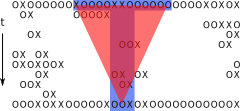
\includegraphics{overview}
    \end{center}
    \caption{
        An overview of the method for a neighbor-dependent model, showing an
        initial sequence on top, a collection of mutations progressing through
        time, and a final sequence.
        The pink trapezoidal region represents the ``range of influence'',
        i.e., possible locations and times at which a mutations is likely
        to affect the mutation outcome at
        the sites of interest (the three sites in the center of the final sequence).
        The blue T shape is called a \emph{T-mer},
        which is how our approximation to the process is parameterized.
        The central, smaller segment of the T is called the \emph{base} of the T-mer.
        The key building block for our method computes the transition probability
        for this subsequence
        conditioned on the ancestral state at the additional \emph{overhang}
        sites of the top of the T.
        \label{fig:overview}
    }
\end{figure}

Before diving into a formal problem specification,
we offer an intuitive explanation of how the method works.
The difficulty of context-sensitive models is that, in principle,
one may have a sequence of events with cascading consequences that involves a lot of the sequence.
In the extreme case, one may have a sequence of mutations from,
say, the left end of the sequence to the right end of the sequence,
such that the probability of each mutation has been changed by that of the previous one.

However, the starting point of the work presented here is that
for typical models such a sequence of events is improbable.
For that reason, we can compute the transition probability for each segment of the sequence
using a local context which,
although bigger than the context which determines the local transition rates,
is much smaller than the entire sequence.
We call the building blocks of this computation \emph{T-mers} (Figure~\ref{fig:overview})
which parameterize transition probabilities for a small section of sequence
(the \emph{base} of the T-mer) based on additional sequence (the \emph{overhang} of the T-mer).
We can then bound the probability that the influence of a mutation
outside the overhang of the T-mer will impact the sites at the base of the T-mer,
which translates into an estimate of approximation error in our calculation of the likelihood.
% note: we are not doing composite likelihood

%%%%%%% %%%%%%%%%%
\section{A general context-dependent model}

Consider a 1-dimensional grid of sites, each of which can take one of a finite set of states,
and that switch randomly between states according to a local set of rules.
We then observe a finite collection of these sites at only a few times,
Suppose that the dynamics are Markov:
writing $\calS$ for the set of possible states
and $X_i(t)$ for the state of site $i$ at time $t$,
we assume that $\{X(t)\}_{t \ge 0}$ is a Markov process on sequences of $L$ states $\calS^L$
for which the probability a given site changes state in a small amount of time
depends only on the sequence of states at nearby sites.

To formalize this notion of local dependence,
first define a \textit{pattern} to mean a contiguous sequence of states,
and let $|u|$ denote the length of a pattern $u$.
Given a sequence $x \in \calS^L$,
let $x_i^{(h)} = (x_i, x_{i+1}, \ldots, x_{i+h-1})$ denote the pattern of $x$ of length $h$ beginning at location $i$.
% Recall we are focusing on finite sequences, and by default, we do not allow patterns to ``hang off'' the end of the sequence.
% This is natural in many situations, but in others we might want to other boundary conditions,
% modeling extant, but unobserved, neighbors.
% We will mention this when necessary.
The dynamics of our stochastic process
are determined by the set of allowed transitions and associated rates:
given two patterns $u$ and $v$ of common length $h$,
saying ``pattern $u$ changes to $v$ at rate $\mu$'' means that
\[
    \P\{ X_i^{(h)}(t+dt) = v \given X_i^{(h)}(t) = u \} = \mu dt + o(dt),
\]
regardless of the location $i$ along the sequence.
If more than one pattern would match to cause the same change, their rates add.
Such a rule is defined by its ``transition triple'' $(\mu,u,v)$,
written as ``$u \to v$ at rate $\mu$''.
A model of context-dependent mutation
is defined by a set of all transition triples,
which we denote $\calT$.

Although our main focus is on nucleotides,
it is informative to consider other, simpler, models as well.
Here is one such example.

\begin{example}[TASEP]
  In the \emph{Totally Asymmetric Simple Exclusion Process}
  describes a set of particles moving among some sites,
  with at most one particle per site.
  Each site is either ``empty'' or ``occupied''
  (0 or 1, respectively),
  and each particle, independently at rate $\lambda$,
  checks whether the site to the right is empty,
  and if so, moves there.
  This process therefore has only one transition triple:

  \begin{center}
    \begin{tabular}{c@{\quad$\to$\quad}c@{\quad at rate\quad }c}
      10  &   01   &  $\lambda$.
    \end{tabular}
  \end{center}

  \noindent
  This only has one parameter.
  If we allow particles to exit from the right and new particles to enter from the left
  (e.g., by adding special symbols for the start and end of the sequence),
  then from observing only starting and ending configurations
  we cannot tell with certainty which particles have moved where,
  so it is not obvious how to estimate the speed.
  However, summing over possible particle movements would allow us to
  compute the likelihood of a given configuration change,
  and so estimate the speed by maximum likelihood
  given an initial sequence, a final sequence and an elapsed time.

\end{example}


To allow more compact specification of models,
we also introduce a ``potential'':
suppose that there is a collection of patterns $\{p_i\}$
such that each occurrence of $p_i$ adds a quantity $e_i$ to the total ``energy'' of a sequence,
and that the rate at which each possible change occurs is modulated by a function of the energy difference the change would produce.
This is natural if transition triples describe \emph{proposed} changes,
and that the probability a proposed change actually occurs depends on how much it affects the energy.

Concretely, let $\calP = \{(p_i, e_i)\}$ be a set of (pattern, energy difference) pairs,
and for any sequence $x$ define
$E(x) = \sum_i e_i\, n(x,p_i)$,
where $n(x,p_i)$ is the number of times the pattern $p_i$ occurs in $x$.
These will affect the rates through a nonnegative function $\phi$:
we declare that if the rate at which $x$ changes to $y$ as computed
from transition triples is $\mu$,
then the actual rate is
\[
    \mu \, \phi\left(E(y) - E(x)\right) .
\]
If $\phi(e)$ is not greater than 1, one way to think about this is that
the transition triples give ``proposed changes'',
but these changes only take effect with probability $\phi(E(y) - E(x))$.
We have described this idea in terms natural for a physics model
in which high energy configurations are disfavored,
however it is also suitable for a population genetics model
in which $\phi$ describes the probability of fixation of a mutant allele
given a certain fitness change from the parent.

\begin{example}[Genomic GC content]
    A genome sequence can be written using A, C, G, and T;
    in the most general model of independent mutation across sites, each of the 12 possible transitions occurs at its own rate.
    Furthermore, in many species
    adjacent, methylated CG dinucleotides (``CpG sites'') have a much higher mutation rate to TG and CA
    than either single nucleotide change under the independent model.
    Embellishing the single-nucleotide model with this additional rate results in the model defined by
    \begin{center}
      \begin{tabular}{c@{\quad$\to$\quad}c@{\quad at rate\quad }cc}
        $x$  &  $y$  &  $m_{xy}$ & for $x, y \in \{\nA,\nC,\nG,\nT\}$ and $x \neq y$ \\
        \nC\nG   &  \nT\nG   &  $\gamma$ & \\
        \nC\nG   &  \nC\nA   &  $\gamma$ &
      \end{tabular},
    \end{center}
    where $\gamma$ is the additional CpG rate above the base mutation rate.
    Note that for a given pair of sequences,
    a change $\nA\nC\nG \to \nA\nT\nG$ could have occurred by a $\nC \to \nT$ mutation
    via the independent-sites model,
    or by a $\nC\nG \to \nT\nG$ mutation;
    in such cases
    the total instantaneous rate at which ACG changes to ATG is the sum of the rates
    (in this example, $\gamma + m_{\nC\nT}$).
    % Although this means there are many possible parameterizations,
    % note that the model is identifiable, not overparameterized.

    Counteracting this trend towards decreased G/C
    is GC-biased gene conversion \citep{glemin2015quantification},
    which acts effectively as a selective pressure in favor of G or C bases.
    We model the evolution of a \emph{single} sequence, not a population of sequences,
    imagining this sequence to be the consensus sequence of the population.
    A new mutation with an effect $s$ on fitness that occurs
    in a population of effective size $N_e$ becomes ubiquitous, rather than dying out,
    with probability approximately $(1-\exp(-2 s))/(1-\exp(-2 s N_e))$ \citep{kimura1962probability}.
    If the mutation occurs at rate $\mu$ per individual,
    the total rate it occurs at in the population is $\mu N_e$.
    GC-biased gene conversion effectively means that sequences with more G/Cs are selected for.
    This is incorporated as follows: set the energy of patterns \nC{} and \nG{} to be $s$,
    so that $E(y)-E(x)$ is the net change in number of G's and C's multiplied by $s$.
    We then expect $s$ to be positive.
    Also, define $\phi(e)$ to be the expected rate of fixations of ``selected'' mutations
    with advantage $e$ relative to the per-individual, per-site mutation rate:
    \begin{align*}
        \phi(e) = N_e (1-\exp(-2e))/(1-\exp(-2eN)).
    \end{align*}
    With these definitions,
    if a given change that occurs with rate $\mu$ would change a sequence $x$ to $y$,
    then $\mu \, \phi(E(y)-E(x))$ is the rate at which the mutation
    appears and successfully takes over in the population.

\end{example}

We close with a final example from statistical physics, to be used later:

\begin{example}[Gibbs sampling of the Ising model]
    In the Ising model, each site is labeled as either ``up'' or ``down'' ($+1$ or $-1$ respectively),
    imagined as a string of $L$ magnetic dipoles,
    and the energy associated with a given state $x$ is $E(x) = - \frac{1}{2} \beta \sum_{i=1}^{L-1} x_i x_{i+1} - \frac{1}{2} \gamma \sum_{i=1}^L x_i$.
    Here $\beta$ controls the strength of coupling between neighboring dipoles,
    and $\gamma$ controls the strength of an external magnetic field
    (and both are scaled by temperature).
    The associated stationary distribution on configurations is proportional to $\exp(-E(x))$.
    The following process, also known as ``Glauber dynamics'', preserves the stationary distribution:
    each site, independently at rate $\lambda$,
    forgets its spin,
    and reconfigures to a state chosen with probability proportional to the stationary probability of the resulting configuration:
    Since $\exp(-E(x))/(\exp(-E(x))+\exp(-E(y))) = 1/(1+\exp(-(E(x)-E(y)))$,
    this is:
    \begin{center}
        \begin{tabular}{c@{\quad$\to$\quad}c@{\quad at rate\quad }c}
          $+$  &   $-$   &  $\lambda$ \\
          $-$  &   $+$   &  $\lambda$
        \end{tabular}
        \qquad and \qquad
        \begin{tabular}{cc}
        pattern  &  energy \\
        $+-$ or $-+$  &   $\beta$ \\
        $+$ &   $\gamma$
        \end{tabular}
    \end{center}
    and
    \begin{align*}
        \phi(e) = \frac{1}{1+\exp(-e)} .
    \end{align*}
\end{example}


\paragraph{The generator matrix}
We now describe concretely how the set of transition rates on patterns determines the transition rate matrix for complete sequences, that is,
the $|\calS|^L \times |\calS|^L$ matrix $G(L)$ whose $(x,y)^\text{th}$ entry gives the instantaneous rate
with which the process in state $x \in \calS^L$ jumps to state $y \in \calS^L$.
Recall that $x_i^{(h)} = (x_i, x_{i+1}, \ldots, x_{i+h-1})$ denotes the subsequence of length $h$ beginning at location $i$.
For each $1\le i \le L$, pattern length $h > 0$, and patterns $u,v \in \calS^h$ define the relation
\[
x \xrightarrow{i,u,v} y \qquad \text{iff} \qquad \begin{cases}
  x_k = y_k \quad &\text{for } k<i \\
  x_{i+j} = u_j \quad &\text{for } 0 \le j < h \\
  y_{i+j} = v_j \quad &\text{for } 0 \le j < h,\ \text{and} \\
  x_k = y_k \quad &\text{for } k\ge i+h ,
\end{cases}
\]
i.e., if $x$ and $y$ match except at positions $i,i+1,\ldots,i+h-1$,
and for those positions $x$ matches with $u$ while $y$ matches with $v$.
\revpoint{2}{3}

As before, let $\calT$ be the set of transition triples for the model.
As noted above, there may be more than one way to mutate a sequence $x$ to get $y$:
for each position $i$, let $J(i,x,y)$ be those transitions in $\calT$ that can be applied at $i$
to change $x$ into $y$, i.e.,
\[
    J(i,x,y) = \{ (\mu,u,v) \in \calT \st x \xrightarrow{i,u,v} y \}.
\]
The rate ${G(L)}_{x,y}$ is then the sum of all transition rates that can take $x$ to $y$,
multiplied by the fitness term,
namely
\begin{align} \label{eqn:G_defn}
    {G(L)}_{x,y} = \phi\left(E(y)-E(x)\right) \, \sum_{i=1}^L \sum_{(\mu, u, v) \in J(i,x,y)}  \mu ,
\end{align}
and if there are no triples $(\mu,u,v)$ with $x \xrightarrow{i,u,v} y$ for some $i$, then ${G(L)}_{x,y}=0$.
To make this the generator matrix for a Markov process,
we also set each $G(L)_{x,x}$ so that rows sum to zero.
Indeed, this matrix is very sparse because for most pairs $(x,y)$ there are no transition triples that can change $x$ into $y$.

In principle, this gives us the transition probabilities for the process by a matrix exponential:
\begin{align} \label{eqn:full_likelihood}
    p_n(t;x,y) := \P\{ X(t) = y \mid X(0) = x \} = {\left(e^{tG(L)}\right)}_{xy} ,
\end{align}
which would then provide a route to parameter estimation.
In practice, the size of these matrices makes direct application obviously impractical for anything but very small $L$.
This paper proposes an alternate strategy.



%%%%%%%%%%%%%%%%%%%%%
\section{Simulation}

First, it will be useful for later proofs to have an explicit construction of the process,
also used for simulation,
using a variant of the ``jump chain representation'', also known as the ``Gillespie algorithm''
or ``uniformization'' \citep{hobolth2009simulation}.
\revpoint{2}{5}
Briefly, this  works by first sampling a homogeneous Poisson process of times and locations of possible changes,
at an appropriate rate $\mu^*$ per site,
and then resolving each possible change in temporal order.
(Note that these ``possible changes'' are different than the ``proposed changes'' described above
in terms of the energy model.)
The rate $\mu^*$ should be the maximum ``local'' rate at which transitions occur, across sites and transition outcome states:
\[
    \mu^*
    % = \max \left\{ \sum_{y \in \calS^L} \sum_{(\mu, u, v) \in J(i,x,y)} \mu \qquad \st x \in \calS^L, \quad 1 \le i \le L \right\} .
    = \max_x \sum_{y \neq x} G(L)_{x,y} .
\]
Note that we do not actually need to construct $G(L)$ to find the maximum rate.
Now sample possible changes:
in a sequence of length $L$, over a time period $t$,
first draw the number of possible changes, $N$,
from a Poisson distribution with mean $\mu^* t L$,
and then choose the times $s_k$ and locations $i_k$
at which possible changes occur uniformly
over $[0, t]$ and $\{1, 2, \ldots, L\}$ respectively.
Order the possible change times, so that
\[
    0 < s_1 < \cdots < s_N < t .
\]
(Note that this is equivalent to saying that possible
changes occur at rate $\mu^*$ independently at each of the $L$ sites.)
Now, suppose we have determined the state just before time $s_k$ to be $X(s_{k-1}) = x$.
Then, the new state $X(s_k)$ is chosen by applying a mutation at position $i_k$
with probability proportional to the corresponding rate, i.e.,
out of the possible transitions $\calT$, transition triple $(\mu(j), u(j), v(j))$ is chosen
with probability
\[
q_j = \begin{cases}
    \mu(j)/\mu^* \qquad & \text{if } x_i^{(|u(j)|)} = u(j)  \\
    0 \qquad & \text{otherwise.}
\end{cases}
\]
The remaining probability $q_0 = 1-\sum_{j=1}^{|\calT|} q_j$
gives the probability that the state remains the same.
(By construction of $\mu_*$, $q_0 \ge 0$.)
If triple $(\mu(j), u(j), v(j))$ is chosen, then
the substring of $x$ matching $u(j)$ that begins at position $i_k$
is replaced with $v(j)$ to produce $X(s_k)$.

For instance, to simulate the TASEP, one has only to let $\mu^*=\lambda$,
and at each possible change
check if at site $i_k$ there is a 1 followed by a 0,
and if so, switch them.


\section{Inference}


The problem at hand is to infer the parameters of the model based on the final state of the model after it has evolved from some known initial state.
% If the sequence is long enough and not too much time has gone by
% this should be feasible -- there should be enough information in our observations to do this reliably.
% If the time is too large, the process may ``saturate'' --
% if there are many changes at most sites, then in at least most models,
% we will lose most information about the dynamics,
% retaining information only about the parameters that affect the stationary distribution.
% In TASEP with any boundary conditions, we lose all information as it approaches stationarity,
% while in the Ising model we have information about the temperature $\beta$ and magnetic field $\gamma$ but not the speed of changes, $\lambda$.
% In the CpG model it is not immediately clear what information is retained.
How can we extract the information?
These are Markov processes, on the state space $\calS^L$,
so the full likelihood function is given by \eqref{eqn:full_likelihood},
but doing anything with the $|\calS|^L \times |\calS|^L$ matrix $G(L)$
is clearly infeasible even for moderately sized $L$.
We can, however, compute \eqref{eqn:full_likelihood} with smaller $G(n)$,
so the first thing that one might think to do is to break the sequence up into many blocks of length $m$,
and treat these as independent.
Then, defining $p_m(t;x,y)$ to be the probability that a string $x$ of length $m$ evolves to string $y$ over time $t$,
we would obtain the approximate likelihood function
\[
  \prod_{k=0}^{n/m} p_m(t;x_{km+1}^{(m)},y_{km+1}^{(m)}) .
\]
However, this ignores dependencies between neighboring blocks,
so it is not clear how good this approximation might be.
% Intuitively, we want to increase the size of the context
% -- and the likelihood thus obtained is asymptotically correct for $m$ large,
% but computationally, we are stuck with small values of $m$.

\begin{figure}
    \begin{center}
        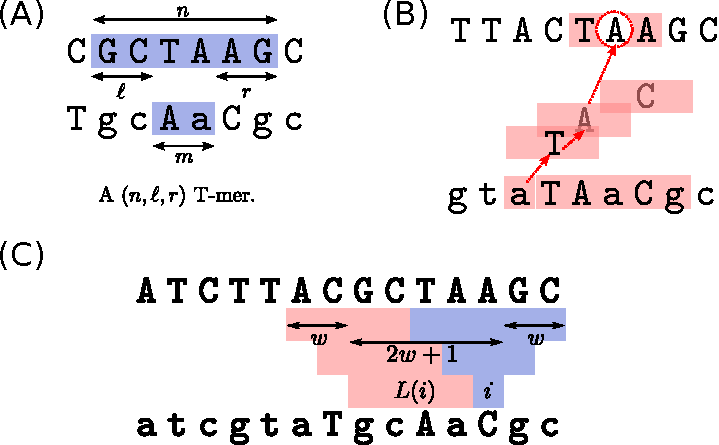
\includegraphics{Tmer-dependency}
    \end{center}
    \caption{
        \textbf{(A)} A $(6,2,2)$ T-mer.
        Nonmutated sites are shown in lower case letters.
        The ``base'' of the T-mer is the lower central
        string of length $m = n - \ell - r$.
        \textbf{(B)}
        The three mutations have extended the influence of the circled \nA{}
        in the initial sequence (top)
        to the six positions colored red in the final sequence.
        The rate of each mutation depends on its' neighboring sites,
        i.e., with a window of width $w=1$.
        Red dotted arrows show the propagation of dependency
        between the circled \nA{}
        and the third site in the final sequence (bottom).
        \textbf{(C)} Diagram of heuristic argument for full likelihood approximation:
        site $i$ depends on the blue squares in $N_i$;
        the sites to the left of this in $L(i)$ are those other sites in $X(t)$
        whose dependency neighborhoods overlap $N_i$.
        Red squares give the dependency neighborhood of $L(i)$,
        so we condition on the row of red and blue sites at the top.
        On the bottom, we have $2w+1$ sites; at the top we have $4w+1$;
        here $w=2$.
        \label{fig:Tmers}
    }
\end{figure}



The key insight we use is that by including neighboring sequence context in the \emph{initial} sequence only,
we can compute \emph{something} correctly,
and that will be sufficient to compute the full likelihood,
at least approximately.
To do this, let $p_{n,\ell,r}(t;x,y)$ for $\ell + r < n$ denote
the probability that an initial subsequence $x$ of length $n$, after time $t$,
is found to match a smaller subsequence $y$ of length $n-\ell-r$, offset by $\ell$ sites
(see Figure \ref{fig:Tmers}).
This central, smaller subsequence is called the ``base'' of the T-mer.
We refer to such patterns as \emph{T-mers}, as depicted in Figure~\ref{fig:Tmers}.
We emphasize that the overhang of the T-mers is typically bigger than the
context-sensitivity width of the underlying model (Figure~\ref{fig:overview}).

These $p_{n,\ell,r}(t;x,y)$ probabilities can be found by marginalizing $p_n$,
summing over the possible initial and final substrings of $x$
(denoted $a$ and $b$):
\begin{align}
    p_{n,\ell,r}(t;x,y)
    &=
    \sum_{a \in \calS^\ell} \sum_{b \in \calS^r} p_n(t;x,a \join y \join b) ,
    \quad
    \text{for}\; x \in \calS^n, \; y \in \calS^{n-\ell-r} ,
    \label{eq:pmMarg}
\end{align}
where $a \join y \join b$ is the sequence composed of concatenating $a$, $y$, and $b$ together in that order.
We expect $p_{n,\ell,r}(t;x,y)$ to be asymptotically correct when $\ell$ and $r$ are large (and $t$ is fixed).
In Appendix~\ref{ss:approx_pf}, we show that this is so, namely that
the probability a given subsequence of length $n$ matching $x$
is later observed to have its center matching $y$
is close to $p_{n,\ell,r}(t;x,y)$, regardless of wider context.
Formally, for each $i$,
\begin{align} \label{eqn:window_approx}
    \P\{ X_{i+\ell}^{(n-\ell-r)}(t) = y \mid X_i^{(n)}(0) = x \}
    \approx
    p_{n,\ell,r}(t;x,y)
    ,
\end{align}
with the approximation getting better for longer $\ell$ and $r$.

Equation \eqref{eq:pmMarg} could then be used to compute a composite likelihood,
which we denote $A_{n, \ell, r}(x,y)$.
This is the product of the probabilities
of transition for all $(n, \ell, r)$ T-mers between $x$ to $y$, i.e.,
with $m = n - \ell - r$,
\begin{align}\label{eqn:composite_like}
    A_{n, \ell, r}(x,y)
        =
        \prod_{i=1}^{L-m+1} p_{n, \ell, r}\left(t;x_i^{(n)}, y_{i+\ell}^{(m)}\right).
\end{align}
To keep notation simple we've ignored the boundaries of the sequence;
to deal properly with these,
on the right-hand side of the equation $\ell$ should be replaced with $\min(\ell, \max(i-1, 0))$,
and $r$ should be replaced with $\min(r, \max(n-i-\ell-m+1, 0))$.


%%%%%%
\subsection{Full likelihood}

What we actually want is the \emph{full likelihood} $\like(y|x)$,
the probability that a given sequence $x$ evolves into another, $y$, over a given period of time.
This full likelihood can be computed as the product of the probability of each site in $y$
given $x$ and all sites in $y$ further to the left.
Defining $x_{<i}=(x_1, \ldots, x_{i-1})$ to be the subsequence to the left of $i$, this is:
\begin{align*}
    \like(y \mid x) &= \prod_{i=1}^L \P\{ Y_i = y_i \given Y_{<i} = y_{<i} \ \text{and}\; X=x \} .
\end{align*}
Each term in this product is the probability of $Y_i$, given all sites in $X$
and all sites in $Y$ to the left of $i$.
It seems reasonable that, similar to equation \eqref{eqn:window_approx} above,
the process at position $i$ should be approximately independent
of distant positions, given the neighboring positions.

Here is a heuristic argument, depicted in Figure~\ref{fig:Tmers}C.
Suppose that $\ell$ is long enough that approximation~\eqref{eqn:window_approx} holds
with $\ell = r$.
Then we know that site $i$ approximately depends only on mutations within distance $\ell$.
Furthermore, the sites up to distance $2 \ell$ to the left of $i$
also depend on these mutations.
We can now use \eqref{eqn:window_approx} to restrict the dependency on $x$.
Recall that the last base of $x_i^{(h)}$ is $x_{i+h-1}$.
So, $x_{i-3\ell}^{(4\ell+1)}$ runs from $i-3\ell$ to $i + \ell$, inclusive, while $y_{i-2\ell}^{(2\ell+1)}$ runs from $i-2\ell$ to $i$, inclusive.
This suggests that the following approximation should be good:
\begin{align} \label{eqn:full_approx}
    \begin{split}
    \P\{ Y_i = y_i \given Y_{<i} \ \text{and}\; X=x \}
    &\approx
        \P\{ Y_i = y_i \given Y_{i-2\ell}^{(2\ell+1)} \;\text{and}\; X_{i-3\ell}^{(4\ell+1)} \}  \\
    &=
        \frac{
            p_{4\ell+1,\ell,\ell}(t; x_{i-3\ell}^{(4\ell+1)}, y_{i-2\ell}^{(2\ell+1)})
        }{
            p_{4\ell+1,\ell,\ell+1}(t; x_{i-3\ell}^{(4\ell+1)}, y_{i-2\ell}^{(2\ell)})
        }.
    \end{split}
\end{align}
\revpoint{2}{6}

Since the full likelihood is a product across sites,
we can then simply express an approximate full likelihood as
a ratio of two composite likelihoods:
\[
    \like(y \mid x) \approx \frac{ A_{4\ell+1, \ell, \ell}(x,y) }{ A_{4\ell+1, \ell, \ell+1}(x,y) }.
\]
% Define $n_\ell(x,y;a,b)$ to be the number of times pattern $a$ is seen in sequence $x$
% matched to pattern $b$ in $y$ at a position offset by $\ell$.
% Then
% \begin{align}
%     \log \like(y|x)
%     &\approx
%         \sum_{a \in \calS^n} \sum_{b \in \calS^{n-2\ell}} n_\ell(x,y;a,b) \log p_{n,\ell,\ell}(t;a,b)
%         -
%         \sum_{c \in \calS^n} \sum_{d \in \calS^{n-2\ell-1}} n_\ell(x,y;c,d) \log p_{n,\ell,\ell+1}(t;c,d)
% \end{align}

See the next section for more discussion of the approximations.

%%%%%
\ubsection{Choice of overhang}

The approximations in~\eqref{eqn:window_approx} and~\eqref{eqn:full_approx} hold
if the overhang, $\ell$, is long enough.
We present intuition about these formulas here, which provides a way to pick the overhang lengths $\ell$ and $r$;
a precise statement is given in Appendix~\ref{ss:approx_pf}.
Suppose that each instantaneous change depends on positions at most $w$ sites away,
and refer to $w$ as the ``window width''.
Then, the mutation process at any particular site
depends on the initial sequence at that site and within distance $w$ on either side\ldots
\emph{and} the outcomes of any mutations that have occurred within that window
(see Figure \ref{fig:Tmers}).

Therefore, the sequence at a particular site may directly affect the process at the neighboring $w$ sites on either side.
If another change happens, say, at the end of this window,
then the indirect effects of this change may extend out to $2w$ sites.
In this way, the influence of the sequence at each site extends outwards, as shown in Figure~\ref{fig:Tmers} --
so if we take the overhangs long enough that this dependency is unlikely to extend to the base of the T-mer,
the approximation will be good.
As we show in Section \ref{ss:approx_pf}, if the overhangs are $\ell = r = kw$,
then the error in approximation \eqref{eqn:window_approx}
is bounded by the probability that there are more than $k$ changes in a given window of length $w$.
Concretely, sites further away than $kw$ only matter if there is a chain of at least $k$ intervening mutations
-- which is unlikely if $k$ is much larger than the expected number.

For instance, in the CpG model the window width is $w=1$
because the process only depends on neighboring sites;
and if the sequence has evolved for time $t$ then we expect no more than a Poisson($\lambda t$) number of changes at each site.
If $\lambda t = 0.75$ ($1-e^{-3/4}=52\%$ of the sequence will have changed!),
then taking $\ell = r = 3$ allows us to compute T-mer probabilities to within an error of 0.007,
since this is the probability that a Poisson with mean 0.75 will be larger than 3.
If $\lambda t = 0.25$ we would do even better with $\ell = r = 2$.

Appendix~\ref{ss:approx_pf} makes this argument more precise.
The argument for the full likelihood is more difficult,
so at present our proposal above remains a conjecture.
To see one difficulty, consider the TASEP model,
with $x_1 = y_n = 1$, and all remaining positions equal to 0.
The full probability of this pair of sequences is very small,
while the conditional probability of $Y_n=1$ given $X=10\cdots0$ and $Y_{<n} = 0\cdots0$
is large since the 1 that initially began in the first position
had to go somewhere.
However, if we do not include the first position in the conditioning,
this conditional probability is very different.
% More generally, it is harder because conditioning on the final sequence $y$
% in effect allows dependencies to propagate back in time as well as forward.
Fortunately, such situations are rare,
and the TASEP model provides the extreme case of dependency propagation.
In practice, we recommend computing the likelihood with equation \eqref{eqn:full_approx}
using successively larger values of $\ell$
to check for convergence.

\paragraph{Boundary conditions} \revpoint{2}{1}
Above, we have chosen to disallow changes whose patterns extend beyond the end of the sequence,
i.e., the pattern $u$ (and hence, also the replacement $v$) of each transition triple
must fit entirely within the existing sequence.
Alternatively, we might assume periodic boundary conditions,
which are natural for the Ising or TASEP models.
Or, if the sequence we consider is embedded within a larger, unknown sequence,
then we might assume a statistical model for the flanking sequence,
averaging over the rates implied by states chosen from a stationary distribution.
Our choice here of ``empty'' boundary conditions
has the nice property that the total rate of changes on a given sub-segment of sequence
is monotonically increasing in the length of the overhang,
which gives us a simple check that the overhang is long enough
(by seeing whether the total rate of change has converged).
However, the software also allows periodic boundary conditions.


%%%%%%%%%%%
\section{Computation}

For inference, we need to compute the $|\calS|^{n} \times |\calS|^m$ matrix $F$ whose $(a,b)^\text{th}$ entry is $p_{n,\ell,r}(t,a,b)$,
for various $t$ (and $m = n - \ell - r$).
This matrix is a projection of the $|\calS|^{n} \times |\calS|^{n}$ matrix whose $(a,c)^\text{th}$ entry is
\begin{align}
    p_{n}(t;a,c) = \left( e^{t G(n)} \right)_{a,c} ,
\end{align}
where $G(n)$ is the sparse $|\calS|^{n} \times |\calS|^{n}$ matrix defined in \eqref{eqn:G_defn}.
The ``projection'' we need just marginalizes over long (i.e., length $n$) patterns $c$ that match the shorter (i.e., length $m$) pattern $b$
as in \eqref{eq:pmMarg}:
if we define the $n \times m$ matrix $U$ so that $U_{cb}=1$ if $c_\ell^{(m)}=b$ and $U_{cb}=0$ otherwise,
then
\begin{align} \label{eqn:Tmer_trans}
    p_{n,\ell,r}(t;a,b) = \sum_{c \in \calS^{n}} \left( e^{t G(n)} \right)_{ac} U_{cb} ,
\end{align}
so in fact we don't need the entire matrix $e^{t G(n)}$,
just the product of this matrix with each of the columns of $U$.
Modern techniques in sparse matrix computation (e.g., Krylov methods) provide efficient ways to do this.

Using the R package expm \citep{R_expm}, this makes computation quite feasible:
with four possible states and $\ell=2$ and $m=1$, so that $G(n)$ is a $1024 \times 1024$ matrix,
computing $e^{t G(5) }$ takes 13 seconds, while computing $e^{t G(5)} U$ takes only 0.3 seconds.
Increasing to $\ell=4$ and $m=1$ or $\ell=3$ and $m=2$ is still feasible, taking $e^{t G(8)} U$ in 42 and 47 seconds, respectively
(and much longer for the whole matrix $e^{t G(8)}$).

% Although we haven't used such tools here, taking the derivative with respect to $t$ can also be performed using sparse matrix operations.


\paragraph{Sparsity and updating $G$}
We can also take advantage of the sparsity of $G$ to perform efficient computation of the likelihood
under many sets of parameters.
Let's assume that the T-mers only allow single-position changes.
First note that in this case $G(n)$ has
$(1+n(|\calS|-1)) |\calS|^{n}$ nonzero entries,
since each of the $|\calS|^{n}$ sequences can change in $n$ places.
This will determine how the computation scales with $n$ and $|\calS|$,
once we precompute a number of things.
Let $g = (g_1, \ldots, g_d)$ be the nonzero entries of $G(n)$, in some fixed ordering;
sparse matrix representations of $G(n)$ store only $g$ along with information about the rows and columns these are found in.
Each $g_i$ is a linear combination of mutation rates $\mu_j$,
multiplied by a function ($\phi$) of a linear combination of energy coefficients $e_j$,
say $g_i = \sum_j A_{ij} \mu_j \phi(\sum_k B_{ik} e_k)$,
so by precomputing the matrices $A$ and $B$ we can update $G(n)$ with new parameter values
using only two matrix multiplications and evaluation of $\phi()$ over a vector.
This remains efficient to perform in interpreted languages such as R,
since each step is carried out by lower-level compiled code (e.g., optimized linear algebra libraries).
% This is true if the boundary conditions are circular, mean-value, or neither.

%%%%%%%%
\section{Phylogenetic inference}

In phylogenetic applications, rather than ``before'' and ``after'' observations,
we get two (or more) observations evolved from a common root.
In the simplest case of two tips we have two processes $X$ and $Y$,
with identical starting states $X(0)=Y(0)$,
observed only at times $t_X$ and $t_Y$ respectively.
At first, one might think to compute probabilities
with a ``long'' sequence at the root and ``short'' sequences at every tip.
However, this does not work out, since the root is unobserved
and short sequences at every tip give us no information about what the root sequence
in the overhangs might be.

Instead, we will compute the probability that
we see (long) pattern $x$ in $X(t_X)$ juxtaposed with (short) pattern $y$ in $Y(t_Y)$,
summing over possible (long) patterns at the root.
Concretely: pick a random location $I$ in the sequence
and let $X_{I-\ell}^{(n)}(0) = \rho_I$ be the (long) pattern seen there at the root.
Write $\pi(z)$ for the frequency of a given pattern $z$ seen there, i.e., $\P\{\rho_I=z\}=\pi(z)$.
% Given the corresponding pattern in $X(t_X)$, the distribution of $\rho_I$ is proportional to
% \[
%     \P\{ \rho_I=z \mid X_{I-\ell}^{(n)}(t_X)=x\} \propto \pi(z) p_{n}(t,z,x) .
% \]
The probability that we see $x$ and $y$ at the random location $I$ is
\begin{align} \label{eqn:phylo_likelihood}
    \P\{X_{I-\ell}^{(n)}(t_X)=x \text{ and } Y_I^{(m)}(t_Y)=y \}
    =
    \sum_{z \in \calS^{n}} \pi(z) \, p_{n,0,0}(t_X;z,x) \, p_{n,\ell,r}(t_Y;z,y) .
\end{align}
Denote this quantity $p_{n,\ell,r}(x, y)$.
This can be computed without much more effort than the simpler case above,
given the frequencies at the root, as described in greater generality below.
These calculations can be done using the same sparse matrix methods as above.
For instance, to compute
\[
    \sum_{z \in \calS^{n}}
        \pi(z) \, p_{n,0,0}(t_X;z,x) \, p_{n,\ell,r}(t_Y;z,y)
    =
    \sum_{z \in \calS^{n}}
    \left( e^{t_X G(n)} \right)_{zx}
    \pi(z)
    \sum_{w \in \calS^{n}} \left( e^{t_Y G(n)} \right)_{zw} U_{wy} ,
\]
we can first compute $\sum_w \left( e^{t_Y G(n)} \right)_{zw} U_{wy}$ as above,
multiply rows by $\pi(z)$, and then matrix multiply by the transpose of $e^{t_X G(n)}$.

We might approximate the full likelihood as follows,
after choosing $n$, $\ell$, and $r$ appropriately (see above).
For the sake of notational simplicity, assume that we have a few positions
of $X$ observed before the start and after then end of the sequence
(so that, e.g., we can refer to $x_{n+1}, \ldots, x_{n+r}$).
\begin{align*}
    \like(x, y)
    &=
    \prod_{i=1}^L
        \P\{ X_{i+r} = x_{i+r},\; Y_i = y_i
            \given X_{<i+r} = x_{<i+r},\; Y_{<i} = y_{<i} \} \\
    &\approx
    \prod_{i=1}^L
        \P\{ X_{i+r} = x_{i+r},\; Y_i = y_i
            \given X_{i-\ell}^{(n-1)} = x_{i-\ell}^{(n-1)},\; Y_{i}^{(m-1)} = y_{i}^{(m-1)} \} \\
    &=
    \prod_{i=1}^L
    \frac{
        p_{n,\ell,r}\left( x_{i-\ell}^{(n)}, y_i^{(m)} \right)
    }{
        p_{n-1,\ell,r}\left( x_{i-\ell}^{(n-1)}, y_i^{(m-1)} \right)
    }
\end{align*}
We expect this to be a good approximation to the true likelihood
when the same conditions above are met, taking $t$ to the be the largest distance
between two taxa in the tree.

\subsection{Phylogenetic pruning}

The general case is a modification of Felsenstein's ``pruning'' algorithm \citep{felsenstein1981evolutionary}.

\begin{figure}
    \begin{center}
    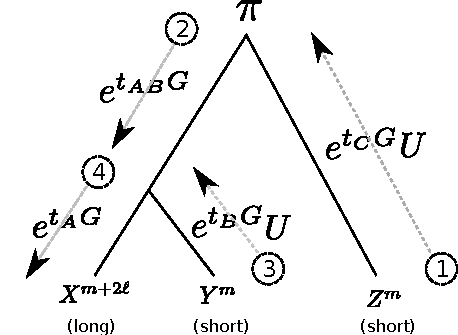
\includegraphics{pruning-schematic}
    \end{center}
    \caption{
        A depiction of the four steps in computing the likelihood
        of finding particular ``short'' subsequences at $Y$ and $Z$
        given the ``long'' subsequence at $X$: see text for details.
        \label{fig:pruning}
    }
\end{figure}

To compute the likelihood on a more complicated tree, consider the following,
with the three-taxon tree of Figure~\ref{fig:pruning} as an example,
where we are counting occurrences of (long) $n$-tuples in taxon $X$,
and (shorter) $m$-tuples in taxa $Y$ and $Z$.
The likelihood in this example is found by summing over the root state (the summation over $u$)
and the interior node ($v$):
\begin{align} \label{eqn:three_taxa_likelihood}
  \begin{split}
    & \P\{X_{I-\ell}^{n}=x \text{ and } Y_I^\ell=y \text{ and } Z_I^\ell=z \} \\
    &\qquad
      =
      \sum_{u \in \calS^{n}} \pi(u) p_{n,\ell,r}(t_C,u,z)
      \sum_{v \in \calS^{n}} p_{n,0,0}(t_{AB},u,v) p_{n,0,0}(t_{A},v,x) p_{n,\ell,r}(t_B,v,y)
  \end{split}
\end{align}
The steps for computing this are then:
\begin{enumerate}

  \item Compute $M_1(u,z) = p_{m,\ell,r}(t_C,u,z)$ (a $|\calS|^{n} \times |\calS|^m$ matrix)

  \item Compute $M_2(v,z) = \sum_{u \in \calS^{n}}  p_{n,0,0}(t_{AB},u,v) \pi(u) M_1(u,z)$ (still a $|\calS|^{n} \times |\calS|^m$ matrix)

  \item Compute $M_3(v,y) = p_{m,\ell,r}(t_B,v,y)$ (a $|\calS|^{n} \times |\calS|^m$ matrix)

  \item Compute $M_4(x,(y,z)) = \sum_{v \in \calS^{n}} p_{n,0,0}(t_{A},v,x) M_2(v,z) M_3(v,y)$ (stored as a $|\calS|^{n} \times |\calS|^{2m}$ matrix).

\end{enumerate}
Then $M_4$ gives all the likelihoods.
This is depicted in the figure, writing $\left(e^{tG}\right)_{ab}$ for the matrix $p_{n,0,0}(t,a,b)$,
and $U$ for the projection matrix that gives $p_{m,\ell,r}(t,a,b) = \left( e^{tG} U\right)_{ab}$.

In total there are $|\calS|^{3m+2\ell}$ possible data combinations.
However, we can reduce dimensionality by only computing probabilities
for certain (more common) patterns: for instance,
one could compute the likelihood for situations where $y$ and $z$ agree (but may differ from $x$
by replacing step (4) with:
\begin{enumerate}

  \item[$4'$.] Compute $M_4(x,w) = \sum_{v \in \calS^{n}} p_{n,0,0}(t_{A},v,x) M_3(v,w) M_4(v,w)$ (stored as a $|\calS|^{n} \times |\calS|^{m}$ matrix).

\end{enumerate}
On a three-taxon tree it is not clear that this is desirable,
but on larger trees it seems likely that we'd want to restrict to combinations with most sites agreeing across the tree.
(Note, however, that one should not first look at the data, observe which combinations $(y,z)$ were most common, and then restrict to only those!)

The algorithm for a general tree is written out in Appendix \ref{ss:pruning_algorithm}.

%%%%%%%%
\subsection{Model fit and model selection}
Fitting a model to nucleotide data will likely require iterative modification of the model.
The difference between observed and expected T-mer counts provide a good assessment of how and whether a model can be improved.
These \emph{residual} counts are usually most usefully computed for T-mers shorter than those used to fit the model,
because the smaller total number of possible T-mers makes it easier to identify the shared patterns.
For each T-mer $(x,y)$, write $O_{x,y}$ for the number of this T-mer observed in the data,
and $E_{x,y}$ for the number expected under the model.
(The expected number is the number of occurrences of $x$ in the initial sequence
multiplied by the probability $p_{n,\ell,r}(t;x,y)$, where $n$ is the length of $x$,
and $\ell$, $r$ are the appropriate overhangs.)
If the T-mers were nonoverlapping, this would form a standard contingency table,
and standard practice would be to divide the residuals by the square root of the expected counts
and compare these to a standard Normal distribution.
However, there are are $n$ possible such tables --
so, we compute normalized residuals as
\begin{align}
    Z_{x,y} = \frac{ O_{x,y} - E_{x,y} }{ \sqrt{n E_{x,y}} },
\end{align}
which is equivalent to averaging the $z$-scores of the $n$ possible tables of nonoverlapping counts.
These can then be compared to a standard Normal distribution.



%%%%%%%
\section{Software}

The methods described here
are implemented in R
and freely available at \url{https://github.com/petrelharp/context}.
The core implementation of T-mer counting and likelihood evaluation
is provided in an R package, \texttt{contextual},
and is supplemented by (documented) code to simulate from context-dependent models
and perform maximum likelihood or Bayesian inference.


%%%%%%%
\section{Results}

%%%%%%%%%%%
\subsection{Stepwise model selection}

We benchmarked the performance of stepwise model selection:
(a) fit a simple model,
(b) choose new motifs to add based on statistically significant residuals,
(c) repeat until no residuals are statistically significant.
To test this method,
we simulated a single sequence of $10^6$ nucleotides
for one unit of time
under the model given in Table \ref{tab:cpg_results},
obtained by embellishing the basic CpG hypermutability model
with the longer mutational motif identified by \citet{harris2015evidence}.
%     \begin{center}
%       \begin{tabular}{c@{\quad$\to$\quad}c@{\quad at rate\quad }cc}
%         $x$  &    $y$  &  $m_{xy}$ & when $x \neq y \in \{\nA,\nC,\nG,\nT\}$  \\
%         \nC\nG     &  \nT\nG     &  $0.4$ & \\
%         \nC\nG     &  \nC\nA     &  $0.4$ & \\
%         \nT\nC\nC  &  \nT\nT\nC  &  $0.1$ & \\
%         \nA\nG\nG  &  \nA\nA\nG  &  $0.1$ &
%       \end{tabular} ,
%     \end{center}
% with $m_{AT}=m_{TA}=0.1$, $m_{CG}=m_{GC}=0.15$, $m_{AC}=m_{TG}=m_{AG}=m_{TC}=0.08$, and $m_{CA}=m_{GT}=m_{CT}=m_{GA}=0.12$.
% Note the model is symmetric under reverse complementation.
The resulting sequences differed at 28.5\% of the sites.

To begin, we fit an unconstrained non-context-dependent
model of single-nucleotide substitution
using a constrained quasi-Newton method (\verb|optim(.., method='L-BFGS-B')| in R).
Recall that for inference, we next need to pick a T-mer shape
with which to compute likelihoods,
and the shape of this T-mer is only determined by the shape of dependencies in the generative model
in that it determines the minimum base and overhang lengths.
We use (5,1,1) T-mers: three sites at the base with an overhang of one on each side.
Since this initial model has no context-dependence,
we could do the first step of model fitting using (1,0,0) T-mers (i.e., single positions),
but for simplicity we use the same T-mer shape for all steps.

After fitting the model, we can look at residuals using any T-mer shape we like.
At this first step, we computed the (2,1,0) and (2,0,1) T-mer residuals,
shown in Table~\ref{tab:resid1}.
The largest residuals are an excess of $\nC \to \nT$ mutations in $\nC\nG$ dinucleotides,
and the reverse-complement pattern ($z$ scores of 88).
Complementing this are deficits of $\nC \to \nT$ mutations in other contexts,
since the $\nC \to \nT$ mutation rate has been fit to be an average across contexts.
This clearly calls for addition of the $\nC\nG \to \nT\nG$ mutation motif (and reverse complement),
which was used in simulating the data.

\begin{table}[ht]
  \begin{center}
        \begin{tabular}{c@{\quad$\to$\quad}c@{\quad at rate\quad }ll}
          \hline
            x & y & truth & MLE \\
          \hline
          \nA  &   \nT           & 0.10 & 0.0996 \\
          \nT  &   \nA           & 0.10 & 0.0982 \\
          \nC  &   \nG           & 0.15 & 0.1505 \\
          \nG  &   \nC           & 0.15 & 0.1497 \\
          \nA  &   \nC           & 0.08 & 0.0784 \\
          \nT  &   \nG           & 0.08 & 0.0792 \\
          \nA  &   \nG           & 0.08 & 0.0798 \\
          \nT  &   \nC           & 0.08 & 0.0795 \\
          \nC  &   \nA           & 0.12 & 0.1202 \\
          \nG  &   \nT           & 0.12 & 0.1196 \\
          \nC  &   \nT           & 0.12 & 0.1198 \\
          \nG  &   \nA           & 0.12 & 0.1193 \\
       \nC\nG  &  \nT\nG         & 0.40 & 0.3978 \\
       \nC\nG  &  \nC\nA         & 0.40 & 0.3978 \\
    \nT\nC\nC  &  \nT\nT\nC      & 0.10 & 0.1033 \\
    \nA\nG\nG  &  \nA\nA\nG      & 0.10 & 0.1033 \\
           \hline
        \end{tabular}
  \end{center}
  \caption{
      True parameter values, and MLE estimates obtained
      from iterative fitting as described in the text to a $10^6$ bp sequence
    evolved to have 28.5\% sequence divergence
    with the above mutational motifs. The transitions $\nC\nG \to \nT\nG$ and $\nC\nG \to \nC\nA$
    were constrained during fitting to be equal (DNA strand symmetry),
    as were the transitions $\nT\nC\nC \to \nT\nT\nC$ and $\nA\nG\nG \to \nA\nA\nG$.
    \label{tab:cpg_results} }
\end{table}

\begin{table}
% cpg-plus-epsilon/32140/base-model-fit-5-3-l1-resids.2.1.l0.tsv
% cpg-plus-epsilon/32140/base-model-fit-5-3-l1-resids.2.1.l1.tsv
    \begin{center}
        \begin{tabular}{ccrrrr}
                $x$ & $y$ & observed &   expected &    residual &  $Z$ \\
                \hline
                \nC\nG  & \nC\_   & 100410   &  120303    & -19892.50   &	-40.55  \\
                \nC\nA  & \nT\_   &  19884   &   28350    &  -8466.43   &	-35.55  \\
                \nC\nT  & \nT\_   &  19998   &   28061    &  -8063.46   &	-34.03  \\
                \nC\nC  & \nT\_   &  23673   &   28177    &  -4503.96   &	-18.97  \\
                \nG\nG  & \nC\_   &  17742   &   19418    &  -1675.92   &	 -8.50  \\
                \nC\nG  & \nG\_   &  18450   &   19478    &  -1028.34   &	 -5.21  \\
                \nA\nG  & \nC\_   &  10968   &   11760    &   -791.73   &	 -5.16  \\
                \hline
                \nG\nT  & \nC\_   &  20490   &   19507    &    983.44   &  4.97   \\
                \nG\nG  & \nT\_   &  20929   &   19278    &   1650.83   &  8.40   \\
                \nC\nC  & \nC\_   & 124149   &  119880    &   4268.52   &  8.71   \\
                \nG\nG  & \nA\_   &  30483   &   28288    &   2195.34   &  9.22   \\
                \nC\nT  & \nC\_   & 126957   &  119389    &   7567.92   & 15.48   \\
                \nC\nA  & \nC\_   & 128673   &  120619    &   8054.46   & 16.39   \\
                \nC\nG  & \nT\_   &  49311   &   28276    &  21034.85   & 88.45   \\
                \hline
                \hline
                \nC\nG  &  \_\nG  &  100803  &  120541  &  -19737.80  &  -40.19 \\
                \nT\nG  &  \_\nA  &   20040  &   28179  &   -8139.45  &  -34.28 \\
                \nG\nG  &  \_\nA  &   20985  &   28288  &   -7302.96  &  -30.70 \\
                \nA\nG  &  \_\nA  &   22929  &   28399  &   -5469.73  &  -22.95 \\
                \nC\nC  &  \_\nG  &   17805  &   19410  &   -1605.01  &   -8.14 \\
                \nC\nT  &  \_\nG  &   10470  &   11684  &   -1214.31  &   -7.94 \\
                \nC\nA  &  \_\nG  &   10839  &   11882  &   -1043.39  &   -6.76 \\
                \hline
                \nT\nC  &  \_\nG  &   20691  &   19509  &    1182.40  &    5.98 \\
                \nC\nC  &  \_\nA  &   20640  &   19160  &    1480.44  &    7.56 \\
                \nT\nC  &  \_\nT  &   30309  &   28320  &    1988.91  &    8.35 \\
                \nA\nG  &  \_\nG  &  127191  &  121450  &    5740.76  &   11.64 \\
                \nG\nG  &  \_\nG  &  127946  &  120977  &    6969.46  &   14.16 \\
                \nT\nG  &  \_\nG  &  127539  &  120512  &    7026.52  &   14.31 \\
                \nC\nG  &  \_\nA  &   49098  &   28186  &   20911.93  &   88.07 \\
                \hline
        \end{tabular}
    \end{center}
    \caption{
        Largest residuals of shape (2,1,0) and (2,0,1) after fitting a model with only ``basic''
        (single-nucleotide) mutations to sequence simulated under the model
        of Table~\ref{tab:cpg_results}, that also includes CpG hypermutability
        as well as $\nT\nC\nC \to \nT\nT\nC$ and $\nA\nG\nG \to \nA\nA\nG$ mutations.
        Note that in the table, the underscore means ``any nucleotide''.
        \label{tab:resid1}
    }
\end{table}

After adding these patterns into the model and re-fitting, we searched for evidence of additional processes happening in the data.
To do so, we calculated length 2 residuals and (3,1,1) T-mer residuals.
Although some of the length 2 residuals had large $z$-scores,
none were as large as those seen in (3,1,1) T-mer residuals,
which are shown in Table~\ref{tab:resid2}.
These show an excess of $\nT\nC\nC \to \nT\nT\nC$ and $\nA\nG\nG \to \nA\nA\nG$ changes,
which were indeed the motifs used when simulating the data.
After adding these in,
% and initializing all parameters to 0.1
no further (3,1,1) T-mer residuals achieved
statistical significance after computing $p$-values with the Gaussian CDF
and applying a Bonferroni correction.
The final parameter values are shown in Table \ref{tab:cpg_results};
parameter estimates differ from the truth by less than 3\% (mostly within 1\%).


\begin{table}
    \begin{center}
        \begin{tabular}{ccrrrr}
            \hline
                $x$ & $y$ & observed &   expected &    residual &  $Z$ \\
                \hline
                \nA\nG\nG  &  \_\nG\_  &  30024  &  32167  &  -2143.48  &  -6.90 \\
                \nT\nC\nC  &  \_\nC\_  &  29910  &  31748  &  -1838.13  &  -5.95 \\
                \nG\nG\nT  &  \_\nA\_  &   5064  &   5549  &   -484.61  &  -3.75 \\
                \nT\nG\nC  &  \_\nA\_  &   4830  &   5172  &   -342.42  &  -2.74 \\
                \nG\nG\nA  &  \_\nA\_  &   5115  &   5462  &   -346.97  &  -2.71 \\
                \nC\nT\nT  &  \_\nG\_  &   2472  &   2717  &   -244.56  &  -2.70 \\
                \nG\nC\nT  &  \_\nT\_  &   4863  &   5192  &   -328.56  &  -2.63 \\
                \hline
                \nA\nT\nG  &  \_\nG\_  &   3225  &   3028  &    196.78  &   2.06  \\
                \nA\nC\nG  &  \_\nA\_  &   4830  &   4588  &    242.29  &   2.06  \\
                \nT\nG\nT  &  \_\nC\_  &   5364  &   5105  &    258.74  &   2.09  \\
                \nG\nA\nG  &  \_\nG\_  &   3285  &   3055  &    229.78  &   2.40  \\
                \nT\nT\nG  &  \_\nC\_  &   2973  &   2752  &    220.59  &   2.42  \\
                \nT\nC\nT  &  \_\nG\_  &   5421  &   5056  &    364.54  &   2.95  \\
                \nT\nC\nC  &  \_\nT\_  &   7590  &   5500  &   2089.79  &  16.26  \\
                \nA\nG\nG  &  \_\nA\_  &   7566  &   5263  &   2302.74  &  18.32  \\
                \hline
        \end{tabular}
    \end{center}
    \caption{
        Largest residuals of shape (3,1,1) after fitting a model with ``basic''
        (single-nucleotide) and CpG mutations to sequence simulated under the model
        of Table~\ref{tab:cpg_results}, that also includes $\nT\nC\nC \to \nT\nT\nC$ and $\nA\nG\nG \to \nA\nA\nG$ mutations.
        Note that in the table, the underscore means ``any nucleotide''.
        \label{tab:resid2}
    }
\end{table}


% df <- structure(list(
%     sim = c(0.1, 0.1, 0.15, 0.15, 0.08, 0.08, 0.08, 0.08, 0.12, 0.12, 0.12, 0.12, 0.4, 0.1),
%     fit = c(0.0996, 0.0982, 0.1505, 0.1497, 0.0784, 0.0792, 0.0798, 0.0795, 0.1202, 0.1196, 0.1198, 0.1193, 0.3978, 0.1033)),
%     .Names = c("sim", "fit"),
%     row.names = c("A->T", "T->A", "C->G", "G->C", "A->C", "T->G", "A->G", "T->C", "C->A", "G->T", "C->T", "G->A", "CG->TG|CG->CA", "TCC->TTC|AGG->AAG"),
%     class = "data.frame")


%%%%%%%%%%%
\subsection{Bayesian inference}

The usage of fast sparse matrix methods described above make likelihood computation fast enough
to use a Metropolis-Hastings-based Markov chain Monte Carlo method
to sample from the posterior distribution on parameters.
To test this,
we evolved $10^6$ sites from the Ising model (described above) with $\lambda=0.5$, $\beta=1.0$, and $\gamma=0.5$
for 1 unit of time,
resulting in around 460,000 possible mutations
and differences at around 186,000 sites between initial and final sequence.
We then placed an Exponential prior with mean 1 on both transitions $+ \to -$ and $- \to +$
(without constraining these to be equal)
and half-Gaussian priors with mean 0 and scale 3 on both $\beta$ and $\gamma$,
counted $(5,3,1)$ T-mers,
and used the \texttt{mcmc} package \citep{geyer2017mcmc} to run a random walk sampler for 10,000 steps
(judged sufficient by examination of diagnostic plots).
We repeated this procedure separately on 61 independently simulated sequences,
and show the resulting credible intervals in Figure~\ref{fig:ising_coverage}.

Posterior medians were within half a percent of the truth for $+ \to -$ and $- \to +$ (corresponding to $\lambda$)
and the temperature ($\beta$), but showed around 2\% error for the magnetic field $\gamma$.
As seen in Table~\ref{tab:ising_coverage},
credible intervals were somewhat too narrow for shorter T-mers,
but $(6,2,2)$ T-mers were long enough with sufficient overhang to produce well-calibrated posteriors.

\begin{table}[ht]
\centering
\begin{tabular}{rrrr}
  \hline
    & (4,1,1) & (5,1,1) & (6,2,2) \\
  \hline
  $\lambda_-$ & 0.61 & 0.63 & 0.96 \\
  $\lambda_+$ & 0.87 & 0.86 & 0.85 \\
  $\beta$     & 0.76 & 0.81 & 0.94 \\
  $\gamma$    & 0.69 & 0.76 & 0.85 \\
   \hline
\end{tabular}
    \caption{
        Posterior coverage of the four parameters of the dynamic Ising model at four different T-mer sizes.
        Shown are the proportion of runs in which the true value fell within the 95\% credible interval,
        for T-mers of length 4, 5, and 6 with overhangs of length 1, 1, and 2 respectively.
        The total number of runs was 61 for $(6,2,2)$ T-mers and 121 for the others.
        \label{tab:ising_coverage}
    }
\end{table}

\begin{figure}
    \begin{center}
        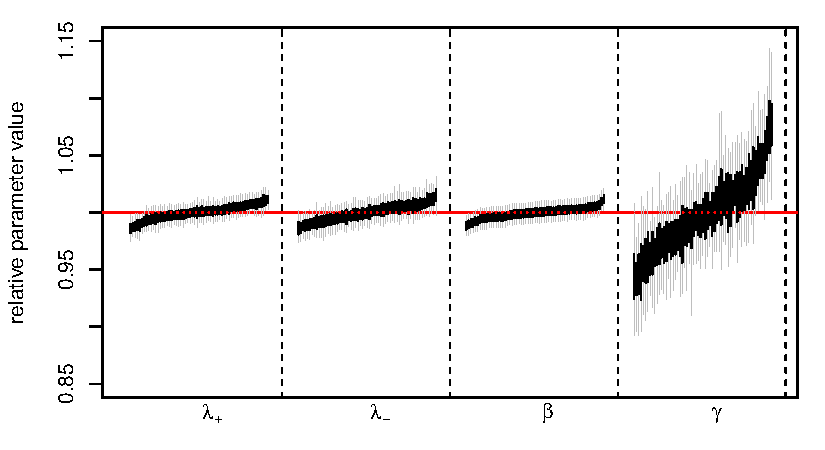
\includegraphics{writeup-plots/coverage_results}
    \end{center}
    \caption{
        Credible intervals for the four parameters of the dynamic Ising model,
        calculated using $(6,2,2)$ T-mers,
        from 61 MCMC runs on independently simulated sequences of $10^6$ spins
        differing at around 18.6\% of the sites.
        Dark bars show the 50\% credible intervals, and lighter grey bars the 95\% credible intervals.
        Values shown are relative parameters, obtained by dividing by the true value.
        \label{fig:ising_coverage}}
\end{figure}


%%%%%%%%%%%
\subsection{Hominid mutation spectrum}

We also applied the method to human--chimpanzee divergence data,
restricting the comparison to putative regulatory sequences,
avoiding the additional constraints of coding sequences.
To do this, we extracted regions in the human (hg38)--chimpanzee (panTro4) alignment % \citep[from the UCSC Genome Browser][]{pantroalign}
according to four types of regulatory feature in the Ensembl Regulatory Build \citep[release 81][]{zerbino2015ensembl}:
``CTCF binding site'', ``enhancer'', ``open chromatin region'', and ``promoter flanking region''.
These were furthermore divided into regions that either did or did not overlap a transcription start or end site of a known gene
from the hg38 Annotations Database \citep{kent2002human}
and filtered for length:
aligned regions below either 3000bp (promoter flanking regions) or 1000bp (all other types).
We then counted T-mers of appropriate length in each of the eight resulting sets of aligned regions, omitting any T-mers that included gaps or repeat-masked positions,
and fit models separately to each of the eight data sets.

We constructed models from three, nested, sets of mutation motifs.
All models are strand-symmetric.
\begin{itemize}
    \item[(basic)]
        Single-base changes, with separate rates for transitions ($\mu_v$),
        \nA$\leftrightarrow$\nT{} ($\mu_{AT}$), \nC$\leftrightarrow$\nG{} ($\mu_{CG}$),
        and other transversions ($\mu_{r}$):
          \begin{center}
            \begin{tabular}{c@{\quad$\to$\quad}c@{\quad at rate\quad }c|c@{\quad$\to$\quad}c@{\quad at rate\quad }c|c@{\quad$\to$\quad}c@{\quad at rate\quad }c}
                \nT  &   \nA   &  $\mu_{AT}$ & \nA  &   \nC   &  $\mu_{r}$ & \nA  &   \nG   &  $\mu_{v}$ \\
                \nA  &   \nT   &  $\mu_{AT}$ & \nC  &   \nA   &  $\mu_{r}$ & \nG  &   \nA   &  $\mu_{v}$ \\
                \nC  &   \nG   &  $\mu_{CG}$ & \nG  &   \nT   &  $\mu_{r}$ & \nT  &   \nC   &  $\mu_{v}$ \\
                \nG  &   \nC   &  $\mu_{CG}$ & \nT  &   \nG   &  $\mu_{r}$ & \nC  &   \nT   &  $\mu_{v}$ \\
            \end{tabular}
          \end{center}

      \item[(CpG)] In addition to the above, an additional CpG rate:
          \begin{center}
            \begin{tabular}{c@{\quad$\to$\quad}c@{\quad at rate\quad }c}
                CG  &   TG   &  $\nu_{CpG}$ \\
                CG  &   CA   &  $\nu_{CpG}$ \\
            \end{tabular}
          \end{center}

      \item[(repair)] In addition to the above, we included a collection of mutation motifs associated with known DNA lesion/repair pathways
          curated from the literature \citep[reviewed in][]{sale2012yfamily,goodman2013translesion,roberts2014hypermutation,cobey2015evolution,goodman2002errorprone}:
          deamination due to repair of UV-induced pyramidine dimers \citep[$\mu_{UV}$,][]{sale2012yfamily,sinha2002uvinduced};
          repair of guanine adducts at CpG sites \citet[$\mu_g$,][]{pfeifer2006mutagenesis};
          deamination by AID \citep[$\mu_\AID$,][]{teng2007immunoglobulin,kasar2015wholegenome};
          deamination by members of the APOBEC family \citep[$\mu_\APOBEC$,][]{alexandrov2013deciphering};
          and repair by error-prone polymerases pol $\eta$ \citep[$\mu_\eta$,][]{alexandrov2013deciphering};
          and pol $\iota$ \citep[$\mu_{\iota}$,][]{roberts2014hypermutation,maul2016polymerase}.
          These are denoted here using ambiguity codes
          \nR{}: \nA{} or \nG{},
          \nY{}: \nC{} or \nT{},
          \nW{}: \nA{} or \nT{}, and
          \nS{}: \nC{} or \nG{};
          so for instance
          ``\nT\nC\nW$\to$\nT\nT\nW''
          means that both
          \nT\nC\nA$\to$\nT\nT\nA{}
          and
          \nT\nC\nT$\to$\nT\nT\nT{}
          share the same mutation rate.
          \noindent
      \begin{center}
          \begin{tabular}{c@{\;\;$\to$\;\;}c@{\;\; {\small at rate}\;\; }c|c@{\;\;$\to$\;\;}c@{\;\; {\small at rate}\;\; }c}
            \nC\nG     &   \nC\nT      &  $\mu_{g}$      & \nA\nA       &   \nA\nG       &  $\mu_{\iota1}$   \\
            \nC\nG     &   \nA\nG      &  $\mu_{g}$      & \nT\nT       &   \nC\nT       &  $\mu_{\iota1}$   \\
            \nT\nC     &   \nT\nT      &  $\mu_{UV}$     & \nA\nA       &   \nG\nT       &  $\mu_{\iota2}$   \\
            \nG\nA     &   \nA\nA      &  $\mu_{UV}$     & \nT\nT       &   \nA\nC       &  $\mu_{\iota2}$   \\
            \nC\nC     &   \nC\nT      &  $\mu_{UV}$     & \nT\nC\nW    &   \nT\nT\nW    &  $\mu_{\APOBEC}$  \\
            \nG\nG     &   \nA\nG      &  $\mu_{UV}$     & \nT\nC\nW    &   \nT\nG\nW    &  $\mu_{\APOBEC}$  \\
            \nC\nC     &   \nT\nT      &  $\mu_{UVd}$    & \nS\nG\nA    &   \nS\nA\nA    &  $\mu_{\APOBEC}$  \\
            \nG\nG     &   \nA\nA      &  $\mu_{UVd}$    & \nS\nG\nA    &   \nS\nC\nA    &  $\mu_{\APOBEC}$  \\
            \nT\nA     &   \nT\nG      &  $\mu_{\eta}$   & \nW\nR\nC\nY &  \nW\nR\nT\nY  &  $\mu_{\AID}$     \\
            \nT\nA     &   \nC\nA      &  $\mu_{\eta}$   & \nR\nG\nY\nS &  \nR\nA\nY\nS  &  $\mu_{\AID}$
        \end{tabular}
      \end{center}

\end{itemize}

The mutational motifs included above are far from complete
-- context-specific affinities and error rates \textit{in vivo}
are not known for most DNA repair pathways --
but neither do they exhaust the hypotheses available in the literature.
For instance, many enzymes act more than once locally when they act,
such as AID \citep{senavirathne2015activationinduced} or error-prone polymerases involved in repair \citep{maul2016polymerase}.

Nevertheless, we find significant effects for a number of biochemically-informed mutation features (Figure~\ref{fig:biochem_results}).
Specifically, we find strong CpG and UV damage effects \citep[][also seen by]{harris2015evidence}.
It may seem tenuous to look for mutational signatures associated with cancer in the germline,
or surprising that UV damage could play a significant role,
but it is reasonable that shared repair machinery might induce similar context-dependent errors.
Other likely sources of error in the germline include the effects of recombination
\citep{arbeithuber2015crossovers,myers2010drive}.


\begin{figure}
    \begin{center}
        \includegraphics[width=\textwidth]{writeup-plots/biochem_mcmc_posteriors}
    \end{center}
    \caption{
        Estimated average mutation rates
        for the motifs in the ``Hominid data'' section
        since the common ancestor of humans and chimpanzee.
        Rates are scaled so that the mean time to common ancestor is 0.001 units --
        if we take this to be 6 million years \citep{scally2012insights,langergraber2012generation}
        then rates are in units of mutations per 6,000 years.
        Shown are posterior medians (points) and 95\% credible intervals (lines, which are quite small in all cases).
        Figure~\ref{sfig:biochem_results_zoom} shows the smaller rates in more detail,
        and Figure~\ref{sfig:biochem_results_relative} shows the rates between categories relative to each other.
        \label{fig:biochem_results}}
\end{figure}

%%%%%%%%%%%%%%%%%%%%
\section{Discussion}

This paper presents a tractable method
for doing statistical inference using observations of a particle model
in which probabilities of change are affected by nearby sites.
Such models appear in many fields, for instance,
as the dynamic counterparts to Markov random fields or spin glass models,
and models of DNA sequence evolution.

The methods described here provide a way to efficiently approximate full likelihoods,
which in many circumstances provide the optimal basis for inference \citep{neyman1933problem},
fast enough to allow Bayesian inference from Monte Carlo sampling.
The method is fast thanks to its dependence on only local neighborhoods
(so the time does not scale with sequence length once T-mer abundances are counted)
and its reliance on sparse matrices whose structure can be precomputed and cached.
It avoids approximations made by previous methods thanks to the use of T-mers
and explicit quantification of the necessary length of the ``arms'' of the T-mers.
We first discuss possible uses of the method,
followed by challenges (and possible solutions).


\paragraph{Other applications}
One class of applications stems from \emph{inference of process} --
where the numerical values of various mutation rates are directly of interest.
For instance, CpG hypermutability depends on the \nC\nG pair being methylated,
an epigenetic modification that has important consequences for gene regulation;
therefore, inference of CpG mutation rates in ancient taxa provides an indirect estimate
of methylation status in extinct organisms.
Similarly, many mutational motifs are thought to be caused by particular enzymes;
inference of relative rates of these motifs
may provide clues as to the activity and evolution of those enzymes.
Furthermore, iterative model building by examining residual motif counts
could provide a powerful way to discover unknown processes
whose action had been obscured by other sources of noise.

In other applications, reconstruction of an unknown sequence may be of interest.
For instance, training data might be used to estimate parameters of a noisy transmission line,
facilitating the later reconstruction of noisily transmitted signals.
Alternatively, multiple observations of independently transmitted copies of a single sequence
(e.g., down a phylogenetic tree)
might be used to estimate the process, and from this infer the original (ancestral) sequence
(or sample from its posterior distribution).
There is no conceptual barrier to applying these methods to lattices in higher dimensions,
such as noisy images or particle systems used to model other physical processes.
However, computational costs will grow with the size of the local neighborhood used
even faster than in one dimension. \revpoint{2}{2}


\paragraph{Limitations}
The model presented assumes that the same process occurs at every location along the sequence,
and that the length of the sequence does not change (no insertions or deletions).
Neither of these assumptions are likely to be true for any data set of DNA sequence;
however, both assumptions are also commonly made in phylogenetics.
Some relaxation of the assumptions is possible -- for instance,
we can easily allow heterogeneity between sites by scaling rates by an overall gamma-distributed random factor \citep{yang1994maximum}.
Insertions and deletions are problematic, however.

Furthermore, we have not been able to put
quantitative bounds on how well we can approximate the full likelihood
with a given T-mer shape.
One reason this is difficult is that there are special cases of initial and final sequence
for which the likelihood is \emph{not} approximable by looking only at T-mer counts;
however, we believe such situations to be rare,
so that the full likelihood can be well approximated on a set of outcomes of high probability.
The TASEP model represents in some ways the worst-case of dependency propagation,
and has an analytic solution \citep{schutz1997exact}.
Further theoretical work in this direction would be welcome.
In practice,
the approximation may be checked by computing the likelihood
using successively longer T-mers,
and checking for convergence as the length (of both base and overhang) increase.


\paragraph{Computation}
The main factor that determines computation time
is the lengths of the T-mers used for inference,
since all computations scale with the number of possible patterns at the long end of the T-mer.
Although the model is efficient enough to deal with fairly long T-mers,
this exponential growth puts hard constraints on the application of the method.
The length of T-mers required to accurately compute the likelihood in most models grows at most linearly
with the mean density of substitution between the initial and final sequence.
This does not in practice greatly increase the length of required T-mer
since substitution densities approaching 100\% are unlikely to be usable in practice
especially if how the sequences align with each other is unknown.
A more serious determining factor of T-mer length is the degree of dependency in the model itself.
For instance, inserting the 13-base pair motif selected against by meiotic drive in primates \citep{myers2010drive}
would require T-mers of width at least 25, and hence vectors of length $4^{25} \approx 1.13 \times 10^{15}$.


\paragraph{Modeling}
Careful building of complex models in this framework may take care,
but no more than in any other class of models (e.g., multivariate linear regression).
It is easy to specify nonidentifiable models --
for instance, all 2mer mutation motifs include the 1mer motifs.
The large number of possible mutation motifs also makes multiple testing an issue;
an unguided approach might include all possible motifs but place a shrinkage prior on their values \citep{bhadra2015horseshoe}.
The converse approach of adding motifs that are overrepresented in the residuals
may be quicker, but entails some degree of arbitrariness in choosing the motifs to add (and in which order).
Finally, inference on trees may be difficult unless the root placement and distribution are strongly constrained:
otherwise, initial investigations suggest the likelihood surface is often strongly ridged --
for instance, increasing the abundance of \nG\ nucleotides at the root while also increasing the mutation rate away from \nG\
can achieve roughly the same result.
However, in phylogenetic applications outgroups can be used to constrain these quantities.

In the genomic context,
if we knew the specific mutational spectrum of each possible repair or copying pathways,
then this framework could be used to rigorously estimate their average usages and impacts.
Despite substantial progress over the past two decades \citep{goodman2013translesion,sale2012yfamily},
this is still far from known.
A promising alternative would be to use the distinct signatures obtained by dimension reduction techniques as in
\citet{alexandrov2013signatures}, \citep{mathieson2017differences} or \citep{shiraishi2015simple} as a proxy for unknown but distinct pathways.



\subsection{Acknowledgements}
The initial impetus for this project came from Matt Dean;
along the way substantial encouragement and useful suggestions were provided by
Will DeWitt, Simon Tavar\'e, Rasmus Nielsen, Graham Coop, Yaniv Brandvain, and Sergey Nuzhdin.
Many thanks are also due to Jessica Crisci for curating the human-chimp data.
The majority of this work was done while PR was at USC.

FAM's work supported by NIH grants R01 AI146028 and U01 AI150747.
Dr.\ Matsen is an Investigator of the Howard Hughes Medical Institute.
PLR's work was supported by NIH award R01HG010774


\bibliography{context-dependence}

\clearpage

\beginsupplement

\appendix

\section{Supplementary figures}

\begin{figure}[h!]
    \begin{center}
        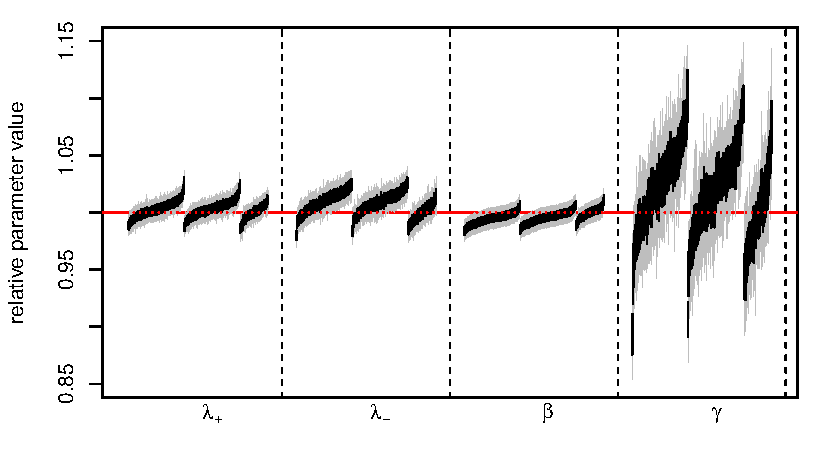
\includegraphics{writeup-plots/coverage_results_all}
    \end{center}
    \caption{
        As in Figure~\ref{fig:ising_coverage}:
        Credible intervals for the four parameters of the dynamic Ising model,
        from MCMC runs on independently simulated sequences of $10^6$ bases
        differing at around 18.6\% of the sites.
        Shown are relative intervals, obtained by dividing by the true value.
        The three groups are left to right, credible intervals obtained from $(4,2,1)$, $(5,3,1)$, and $(6,2,2)$ T-mers:
        note that only the longest $(6,2,2)$ T-mers provide well-calibrated coverage (Table \ref{tab:ising_coverage})
        and do not show bias.
        \label{fig:all_ising_coverage}}
\end{figure}

\begin{figure}
    \begin{center}
        \includegraphics[width=\textwidth]{writeup-plots/biochem_mcmc_posteriors_zoomed}
    \end{center}
    \caption{
        As in Figure \ref{fig:biochem_results}, but with reduced vertical axis range
        to see in more detail:
        estimated average mutation rates
        for the motifs in the ``Hominid data'' section
        since the common ancestor of humans and chimpanzee.
        Rates are scaled so that the mean time to common ancestor is 0.001 units --
        if we take this to be 6 million years \citep{scally2012insights}
        then rates are in units of mutations per 6,000 years.
        Shown are posterior medians (points) and 95\% credible intervals (lines).
        \label{sfig:biochem_results_zoom}}
\end{figure}

\begin{figure}
    \begin{center}
        \includegraphics[width=\textwidth]{writeup-plots/biochem_mcmc_posteriors_relative}
    \end{center}
    \caption{
        As in Figures \ref{fig:biochem_results} and \ref{sfig:biochem_results_zoom},
        but where each rate is divided by the mean rate across all eight categories
        (as well as the 95\% credible interval endpoints).
        \label{sfig:biochem_results_relative}}
\end{figure}

\clearpage

%%%%
\section{Proof of the approximation}
\label{ss:approx_pf}

First we quantify and prove the approximation \eqref{eqn:window_approx}.
The basic idea is that the probability is only in error if there is a chain of mutations
that create a dependency between the base of the T-mer and the flanking sequence.
To simplify the argument, first assume that all transition triples
change only a single, central site in the pattern,
taking into account context on each side of maximum length $w$.
(For instance, a trinucleotide model in which the flanking sites on each side
affect the mutation rate of the central site has $w=1$.)

Recall that, as described in the ``Simulation'' section,
we may represent the process by first laying down a homogeneous Poisson process
with rate $\mu^*$ per site of ``potential mutations'',
where $\mu^*$ is the maximum possible mutation rate,
and then resolving these appropriately.
(In particular, the times and locations of these potential mutations are chosen uniformly.)
Suppose a possible change occurs at site $i-w$, at time $t$,
which therefore might result in a change in mutation rate at site $i$.
To resolve this, we need to know the outcome of any other potential changes
that might change the sequence between $i-w$ and $i + w$.
Consider those that might happen only to the right of $i$,
thus extending the sequence on which the change depends to the right.
The number of such potential changes is Poisson with mean $\mu^* w t$;
if this number is nonzero, then
this extends the amount of sequence on which the change at site $i$ depends
by a uniform number between $1$ and $w$.
If one occurs, say at time $0 < s < t$,
then any further potential changes that occur between time 0 and time $s$
in the $w$ sites to the right of this older potential change
will again extend the range of dependency.
Putting this together, the amount of sequence to the right of a site
on which a mutation at that site depends
is bounded by the compound Poisson process $\sum_{k=1}^N W_k$,
where $N$ is Poisson with mean $\mu^* w t$
and each $W_k$ is independent and uniform on $\{1, 2, \ldots, w\}$.

Now consider the probability of interest,
\begin{align*}
    \P\{ X_{i+\ell}^{(n-\ell-r)}(t) = y \mid X_i^{(n)}(0) = x \} .
\end{align*}
This probability can be written as a sum over all possible arrangements
and resolutions of potential changes.
Our approximation, $p_{n,\ell,r}(x,y)$ is the probability that would be obtained
by ignoring any potential changes that rely on context outside of the $n$-sequence $x$.
So, if $A$ is the event that the final subsequence $y$
depends on sequence outside of $x$ due to potential changes,
then
\begin{align*}
    \left|
        \P\{ X_{i+\ell}^{(n-\ell-r)}(t) = y \mid X_i^{(n)}(0) = x \}
        -
        p_{n,\ell,r}(x,y)
    \right|
    \le \P\{A\} .
\end{align*}
Since the size of the dependency window is a compound Poisson process,
we can bound $\P\{A\}$ using the following lemma:

\begin{lemma}
    Let $V = \sum_{j=1}^N W_j$,
    where $N$ is Poisson with mean $\lambda$
    and each $W_j$ is independent and bounded between 0 and $w$.
    Then for $k \ge 1$,
    \begin{align}
        \P\{ V > k w \}
        \le
        \frac{\lambda^{k+1}}{(k+1)!} .
    \end{align}
\end{lemma}

% # what's this bound look like and how's it compare to a Chebyshev bound
% # that uses the variance of W
%
% ub1 <- function (w, lam, ell=1:10) {
%   k1 <- ceiling(ell/w)
%   return( lam^(k1+1) / factorial(k1+1) )
% }
% # the Chebyshev bound never does better
% ub2 <- function (w, lam, ell=1:10) {
%   k2 <- (ell - lam * (w+1) / 2) / w
%   return( lam * (w+1) * (2*w+1) / (6 * w^2 * k2^2) )
% }
% wvals <- c(1, 2, 3)
% ub1mat <- sapply(wvals, ub1, lam=0.75)
% ub2mat <- sapply(wvals, ub2, lam=0.75)
% matplot(ub1mat, type='l', lty=1)
% matlines(ub2mat, type='l', lty=2)
% legend('topright', lty=1, col=seq_along(wvals), legend=sprintf("w=%d", wvals))

\begin{proof}
    First note that $\P\{V > kw\} \le \P\{N > k\}$.
    Now, use the fact that if $f(n) = n (n-1) \cdots (n-k) / (k+1)!$
    then $f(n) = 0$ for integers $0 \le n \le k$ and $f(n) \ge 1$ for $n > k$,
    and so $\P\{N > k\} \le \E[f(N)]$.
    Now, $\E[f(N)] = \lambda^{k+1} / (k+1)!$ via direct calculation or the
    formula for the $k+1$st factorial moment for the Poisson distribution.
\end{proof}

Putting this together,
we find that
\begin{align*}
    \left|
        \P\{ X_{i+\ell}^{(n-\ell-r)}(t) = y \mid X_i^{(n)}(0) = x \}
        -
        p_{n,\ell,r}(x,y)
    \right|
    \le
    \frac{
        2 (\mu^* t)^{k+1}
    }{
        (k+1)!
    } .
\end{align*}
Here, the factor of 2 comes from the two sides (to the left and right) of the base of the T-mer.

The argument applies to more general transition triples,
with $w$ set equal to the maximum distance
from a position that is changed to the edge of the context
across all transition triples.




\section{Pruning algorithm}
\label{ss:pruning_algorithm}

Fix one tip of the tree, $a$, to be the taxa where we count ``long'' sequences, let $\rho$ be the root, and let $b_1, \ldots, b_n$ be the remaining tips,
where we observe ``short'' sequences.
Let $v_0=\rho, v_1, \ldots, v_\ell = a$ be the path from the root down to $a$,
let $u_1, u_2, \ldots, u_m$ be the remaining internal nodes,
and for each $v_i$ let $u(v_i)$ be the offspring of $v_i$ that is not one of the other $v$.
For each node in the tree,
we will compute a matrix of probabilities:
for nodes not on the path from $a$ to the root,
we compute the chance that each ``long'' sequence observed at that node
is matched by each possible combination of ``short'' sequences on the tips of the tree below it.
For nodes on the path from $a$ to the root, we compute the probability of observing
each ``long'' sequence at that node, along with the combinations of ``short'' sequences
on all tips further away from $a$ (i.e., below that node if it was rooted at $a$).
For a node $w$ this will be stored as a $|\calS|^{n} \times |\calS|^{cm}$ matrix, denoted $M(w)$,
where $c$ is the number of tips for which $w$ lies on the path from $a$ to the tip.
Rows of $M(u_j)$ sum to 1,
while each entire matrix $M(v_i)$ sums to 1;
the difference being that $M(v_i)$ sums over the prior at the root,
and $M(u_j)$ takes the value at $u_j$ as given.
Below, we index columns of $M(u)$ by lists of short patterns,
and leave the specific ordering to implementation.
(For instance, if $c=2$ then a generic entry is $M(u)_{x,(y,z)}$,
where the long pattern $x$ indexes the rows and the pair of short patterns $(y,z)$ indexes the columns;
in the software all matrices retain column names making this unambiguous.)

Let $t(w)$ be the length of the branch above node $w$, for $w \neq \rho$,
and denote by $G^T$ the transpose of $G$.

\begin{enumerate}

  \item Set $M(b_i) = U$ for each $b_i$.

  \item While there are $u_j$ whose children $w_1$ and $w_2$ both have matrices computed, let
        \begin{align}
          M(u_j)_{x,(y,z)} = \left( e^{t(w_1) G} M(w_1) \right)_{x,y} \left( e^{t(w_2) G} M(w_2) \right)_{x,z} .
        \end{align}

  \item Let
    \begin{align}
      M(\rho)_{x,y} = \pi(x) \left( e^{t(u(\rho)) G} M(w(\rho)) \right)_{x,y}.
    \end{align}

  \item For each $1 \le k < \ell$, let
        \begin{align}
          M(v_k)_{x,(y,z)} = \left( e^{t(v_k) G^T} M(v_{k-1}) \right)_{y,x} \left( e^{t(u(v_k)) G} M(u(v_{k-1})) \right)_{x,z}  .
        \end{align}

  \item Finally, let
    \begin{align}
      M(a)_{x,y} = \left( e^{t(a) G^T} M(v_{\ell-1}) \right)_{x,y}  .
    \end{align}

\end{enumerate}

%%%%%%%%%%%%%%%%%
\includereviews

\end{document}
